\documentclass[10pt]{beamer}
\usetheme{Malmoe}
\colorlet{beamer@blendedblue}{green!40!black}
\setbeamertemplate{navigation symbols}{}
\newcommand*\oldmacro{}%
\let\oldmacro\insertshorttitle%
\renewcommand*\insertshorttitle{%
\oldmacro\hfill%
\insertframenumber\,/\,\inserttotalframenumber}

\usepackage{caption}
\usepackage{hyperref}
\usepackage[makeroom]{cancel}
\usepackage{ amssymb }
\usepackage{appendixnumberbeamer}
\usepackage{graphicx}


\begin{document}
\title{Search for Flavor Changing Neutral Currents in Top Quark Decays}
\subtitle{$t \rightarrow q \gamma$}
\author[Barkeloo, Comprehensive Exam]{Jason Barkeloo}

\titlegraphic{
\includegraphics[width=4cm]{../ATLAS-Logo-Ref-RGB.png}\hspace*{2.75cm}~%
   
\includegraphics[width=4cm]{../uo_logo_green_on_white_2.jpg}
}

\date{November 30, 2017}
\frame{\titlepage}
\frame{\frametitle{Table of Contents}\tableofcontents[hidesubsections]}
%\frame{\frametitle{Table of Contents}\tableofcontents[currentsection,hideothersubsections]}
%%%%%%%%%%%%%%%%%%%%%%%%%%%%%%%%%%%%%%%%%%%%%%%%%%%%%%%%%
\section{Background}
\subsection{The Standard Model}

%%%%%%%%%%%%%%%%
\frame{\frametitle{The Standard Model}
\begin{figure}
	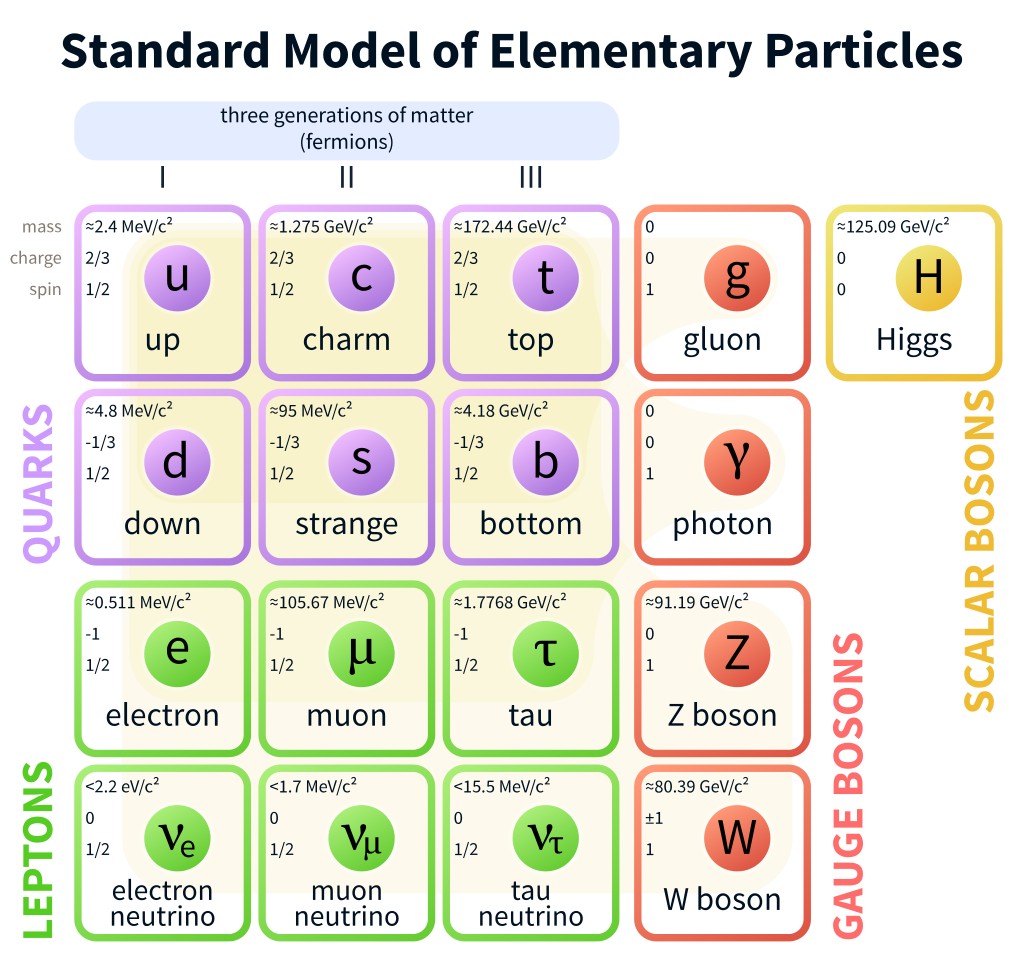
\includegraphics[width=4.8cm]{../../Thesis/ThesisImages/SMParticles.png}
	\captionof{figure}{\href{https://en.wikipedia.org/wiki/Standard_Model}{List of standard model particles}}
\end{figure}
\begin{itemize}
\item Our current theory that attempts to explain everything
	\begin{itemize}
	\item Experimentally precise and well behaved
	\item Very few exceptions (i.e. Neutrino Mass, Matter-Antimatter Asymmetry, Dark Matter Abundance)
	\end{itemize}
	\vspace{\baselineskip}
\end{itemize}
}

\subsection{The Top Quark}

%%%%%%%%%%%%%%%%%%%
\frame{\frametitle{The Top Quark}
\begin{itemize}
\item Heaviest fundamental particle, $172.5 GeV$
\item Lifetime $5x10^{-25}s$, decays before hadronization
	\begin{itemize}
	\item Allows us to study the decay of a single quark
	\end{itemize}
\end{itemize}
\begin{figure}
	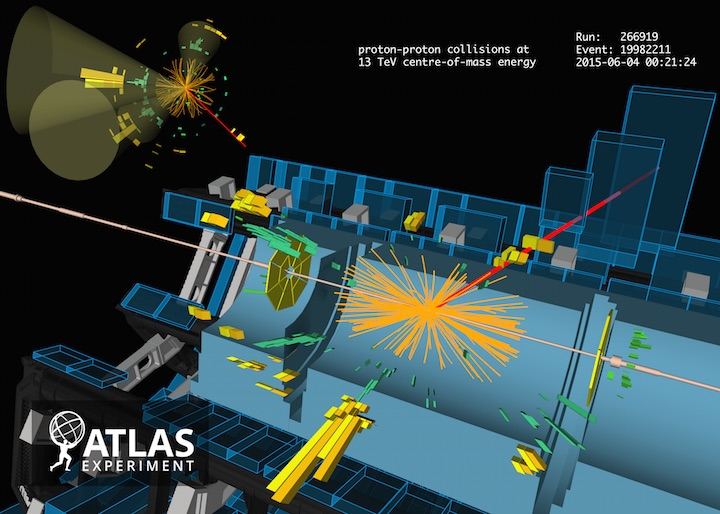
\includegraphics[height=0.5\textheight]{../../Thesis/ThesisImages/ttbarevent.png}
	\captionof{figure}{$t\bar{t}$ event in the ATLAS detector}
\end{figure}
}

\frame{\frametitle{Top Quark Pair Production}
\begin{itemize}
\item Leading order processes for top quark production
	\begin{itemize}
	\item Quark-antiquark annihilation $\approx 10\%$
	\item Gluon-gluon fusion $\approx 90\%$
	\end{itemize}
\end{itemize}
\centering

	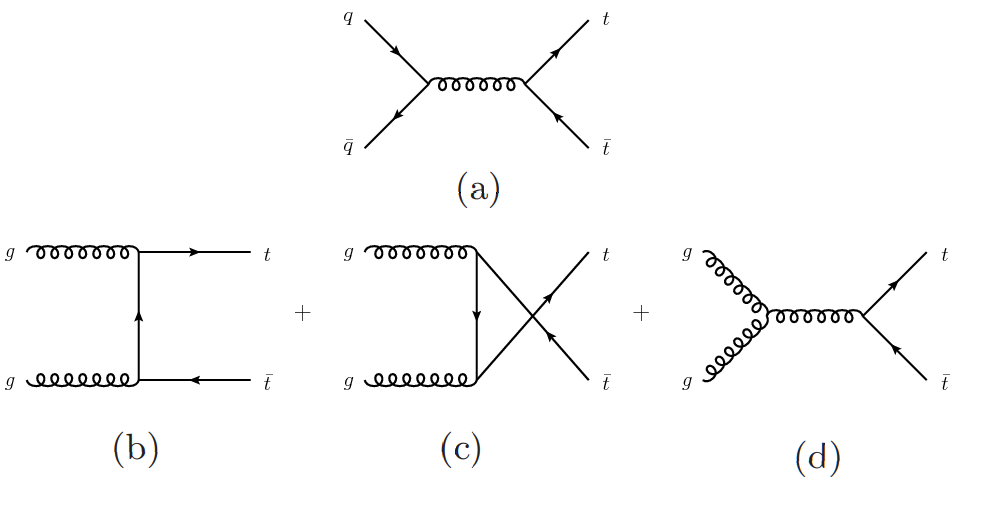
\includegraphics[height=0.5\textheight]{../../Thesis/ThesisImages/Theory/LOPairProdDiags.png}
	\captionof{figure}{Leading order $t\bar{t}$ diagrams}
}

\frame{\frametitle{Top Quark Pair Production}
\begin{itemize}
\item At $\sqrt{s}=13TeV$ for $m_{t}=172.5GeV$, $\sigma_{t\bar{t}} = 831.76pb$
\end{itemize}
\centering
	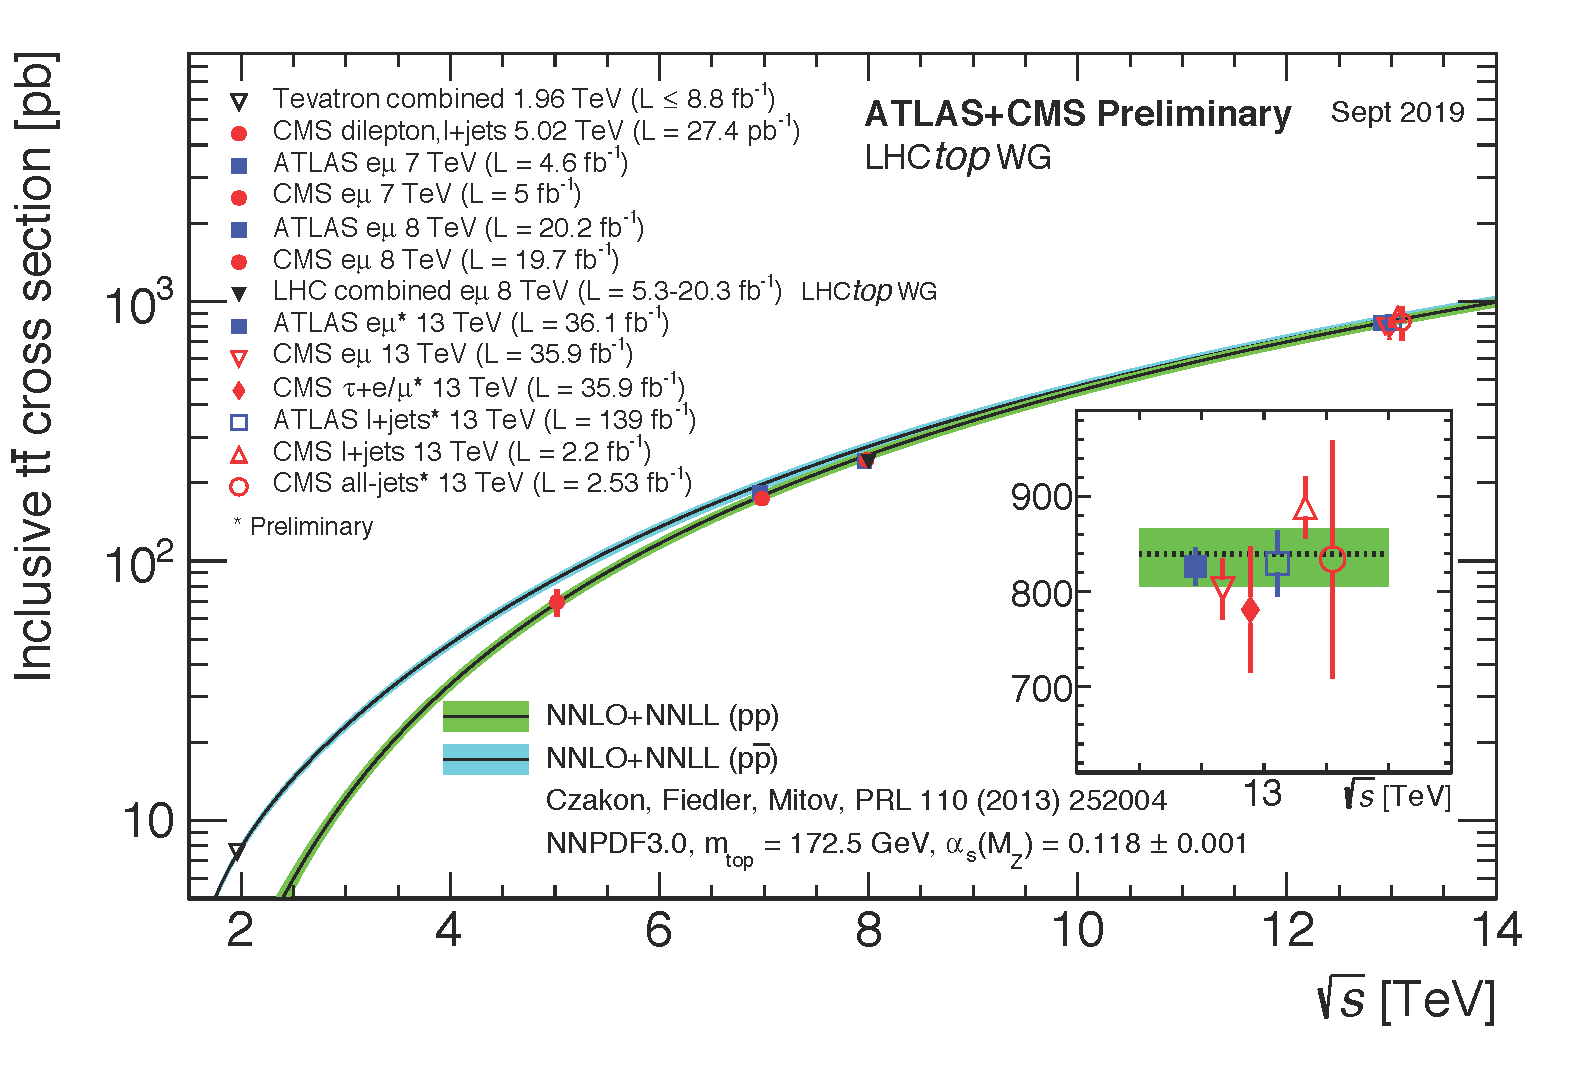
\includegraphics[height=0.7\textheight]{../../Thesis/ThesisImages/Theory/ttprodxsec.png}
	\captionof{figure}{$t\bar{t}$ production cross section \href{https://twiki.cern.ch/twiki/bin/view/LHCPhysics/LHCTopWGSummaryPlots}{[TopWGSummaryPlots]}}
}

\frame{\frametitle{Top Quark Decays}
\begin{columns}
\begin{column}{0.5\textwidth}
\begin{itemize}
\item Standard model top branching ratio to bW $\simeq 100\%$
\end{itemize}
\centering
 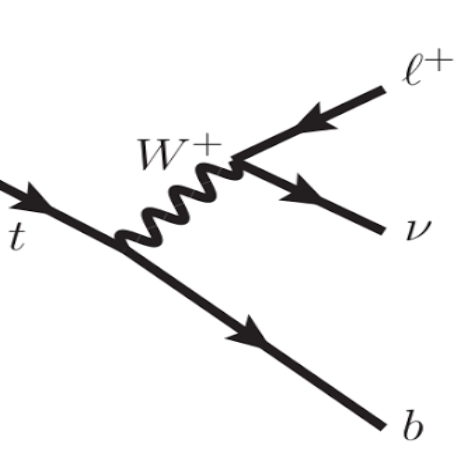
\includegraphics[width=0.7\textwidth]{../../Thesis/ThesisImages/topdecay.png}
 \captionof{figure}{Leptonic final state diagram for a top decay}
\end{column}
\begin{column}{0.5\textwidth}  %%<--- here
     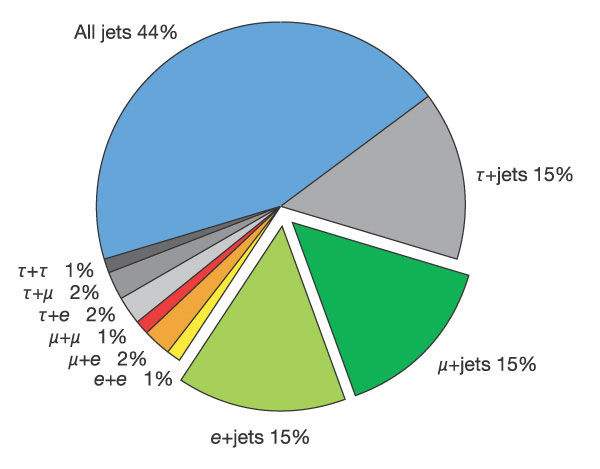
\includegraphics[width=1.1\textwidth]{../../Thesis/ThesisImages/Theory/topdecayproducts.jpg}
    \captionof{figure}{Top quark pair decay final states \href{https://images.nature.com/full/nature-assets/nature/journal/v429/n6992/images/nature02589-f2.2.jpg}{[Nature]}}
\end{column}
\end{columns}
}

\frame{\frametitle{Top Quark Decays in the SM}
\centering
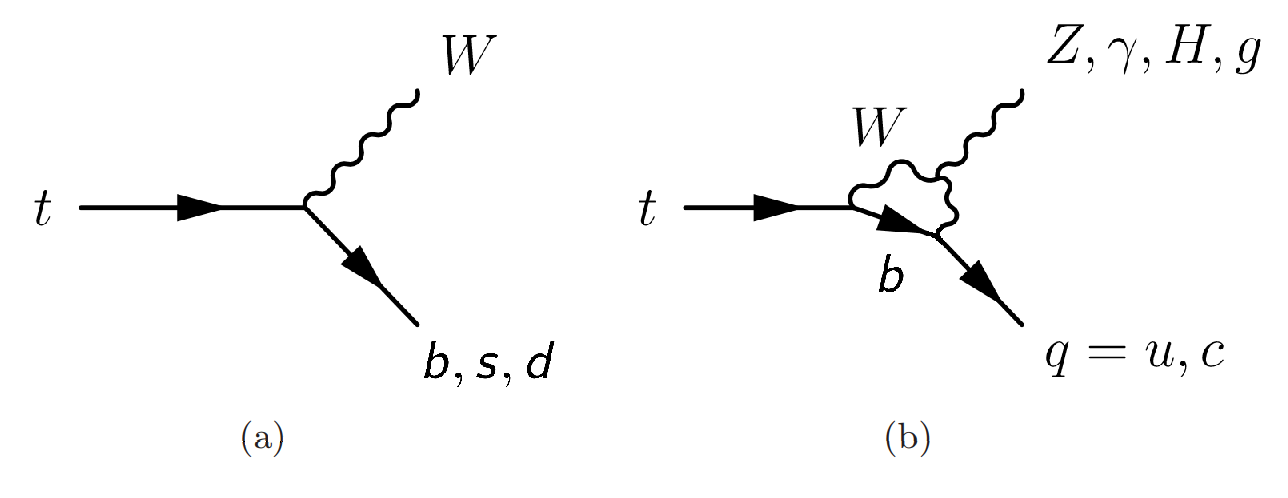
\includegraphics[width=1.\textwidth]{../../Thesis/ThesisImages/Theory/SMTopDecays.png}

\begin{columns}
\begin{column}{0.5\textwidth}
\begin{itemize}
\item $t\rightarrow b W \approx 99.83\%$
\item $t\rightarrow s W \approx 0.16\%$
\item $t\rightarrow d W \approx 0.01\%$
\end{itemize}
\end{column}
\begin{column}{0.5\textwidth}
\begin{itemize}
\item $t\rightarrow q_{u,c} X\approx 10^{-17} - 10^{-12}$
\end{itemize}
\end{column}
\end{columns}

%\feynmandiagram [small,horizontal=a to b] {
%  a [particle=\(t\)] -- [fermion] b ,
% f1 [particle=\({b,s,d} \)] -- b -- [boson] f2 [ particle=\(W\)],
%};
}
%
%%%%%%%%%%%%%%
%\subsection{Historical Background}
%
%\frame{\frametitle{GIM Mechanism}
%\begin{itemize}
%\item Cabibbo model - 3 quarks (u, d, s)
%\item Studies of kaon decays showed the existence of $K^+ \rightarrow \mu^+ \nu_\mu$ but an absence of predicted $K_{L}^0 \rightarrow \mu^+ \mu^-$
%\item Even in the absence of a tree level decay $K_{L}^0$ decay the box diagram would be possible through an exchange of W bosons
%\item Weak neutral current interactions in the uds model  have the form
%\[
%u\bar{u}+ (d\bar{d}\cos^2\theta_C+s\bar{s}\sin^2\theta_C)) +(s\bar{d} + d\bar{s})sin\theta_C cos\theta_C
%\]
%\end{itemize}
%\centering
%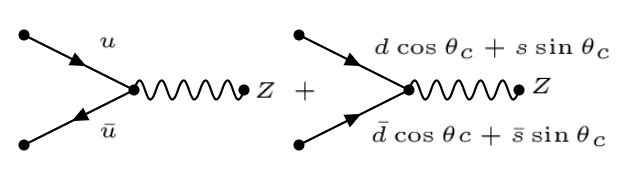
\includegraphics[width=0.45\textwidth]{../../ThesisImages/gimdeltaSa.png}
%}
%
%\frame{\frametitle{GIM Mechanism}
%\centering
%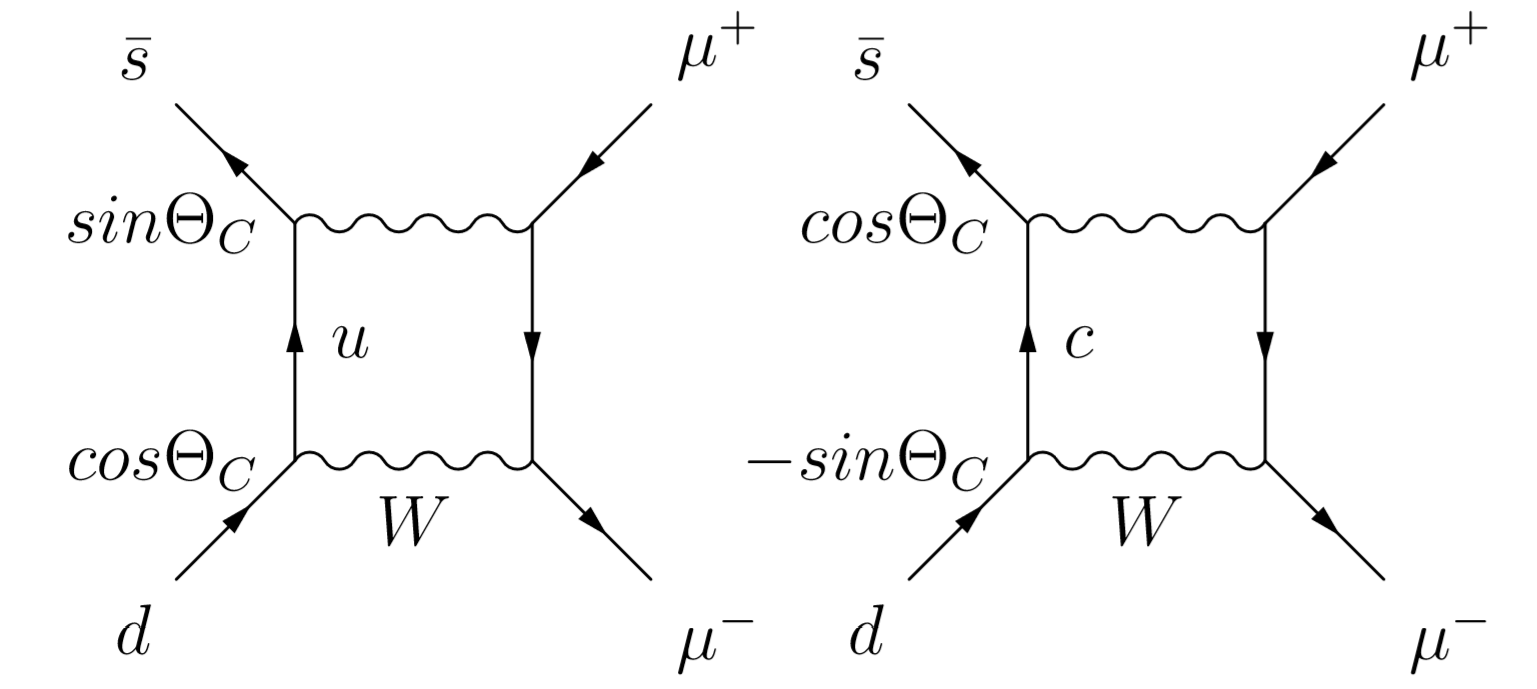
\includegraphics[width=.6\textwidth]{../../ThesisImages/GIMDiagrams.png}
%
%\begin{itemize}
%\item Glashow, Iliopoulos, and Maiani \href{https://journals.aps.org/prd/abstract/10.1103/PhysRevD.2.1285}{[Phys. Rev. D (1970)]} propose a machanism through which FCNCs are suppressed in loop diagrams
%	\begin{itemize}
%	\item Introduction of charm quark
%	\end{itemize}
%\item Kaon decays imply no neutral current/natural suppression of neutral current
%\end{itemize}
%}
%
%\frame{\frametitle{GIM Mechanism}
%\centering
%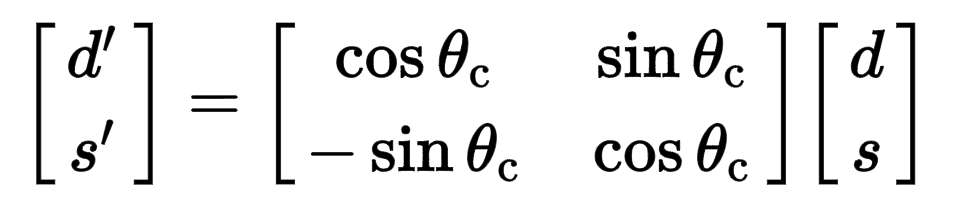
\includegraphics[width=.4\textwidth]{../../ThesisImages/cabibboangle.png}
%\begin{itemize}
%\item The addition of the charm changes our weak neutral current interactions
%\item With four quarks the weak neutral interactions now have the form:
%\[
%u\bar{u} + c\bar{c} + (d\bar{d}+s\bar{s}) \cos^2\theta_C + (s\bar{s} + d\bar{d})\sin^2\theta_C +(s\bar{d} + d\bar{s} - d\bar{s} - s\bar{d})sin\theta_C cos\theta_C
%\]
%\item Flavor changing neutral current diagrams cancel out at tree level (as $m_{c} \rightarrow m_{u}$)
%\end{itemize}
%\centering
%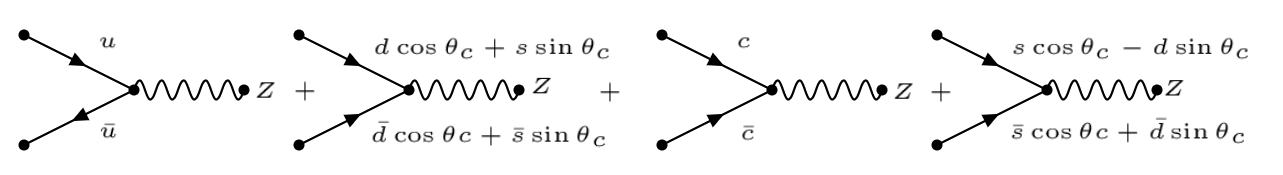
\includegraphics[width=0.9\textwidth]{../../ThesisImages/gimdeltaS.png}
%}
%
%
%\frame{\frametitle{CKM Matrix}
%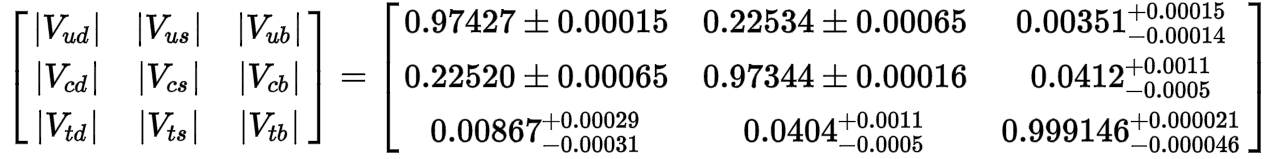
\includegraphics[width=1.\textwidth]{../../ThesisImages/CKMMatrix.png}
%\captionof{figure}{CKM Matrix}
%\begin{itemize}
%\item Decay rates proportional to $|V_{tX}|^2$
%\item Top decay through a $W^{\pm}$ boson is a charged current interaction. 
%\item Flavor changing processes are proportional to off-diagonal elements of the CKM matrix
%\item GIM/CKM suppression of these FCNC processes in the Standard Model make them unlikely to be seen without some new physics
%\end{itemize}
%}
%
%
%
%%%%%%%%%%%%%%%%%%%%%%%%%%%%%%%%%%%%%%%%%%%%%%%%%%%%%%%%%%%%%%%%%%%%%

\subsection{Theory Predictions and Experimental Limits}


\frame{\frametitle{Top Flavor Changing Neutral Currents (FCNCs)}
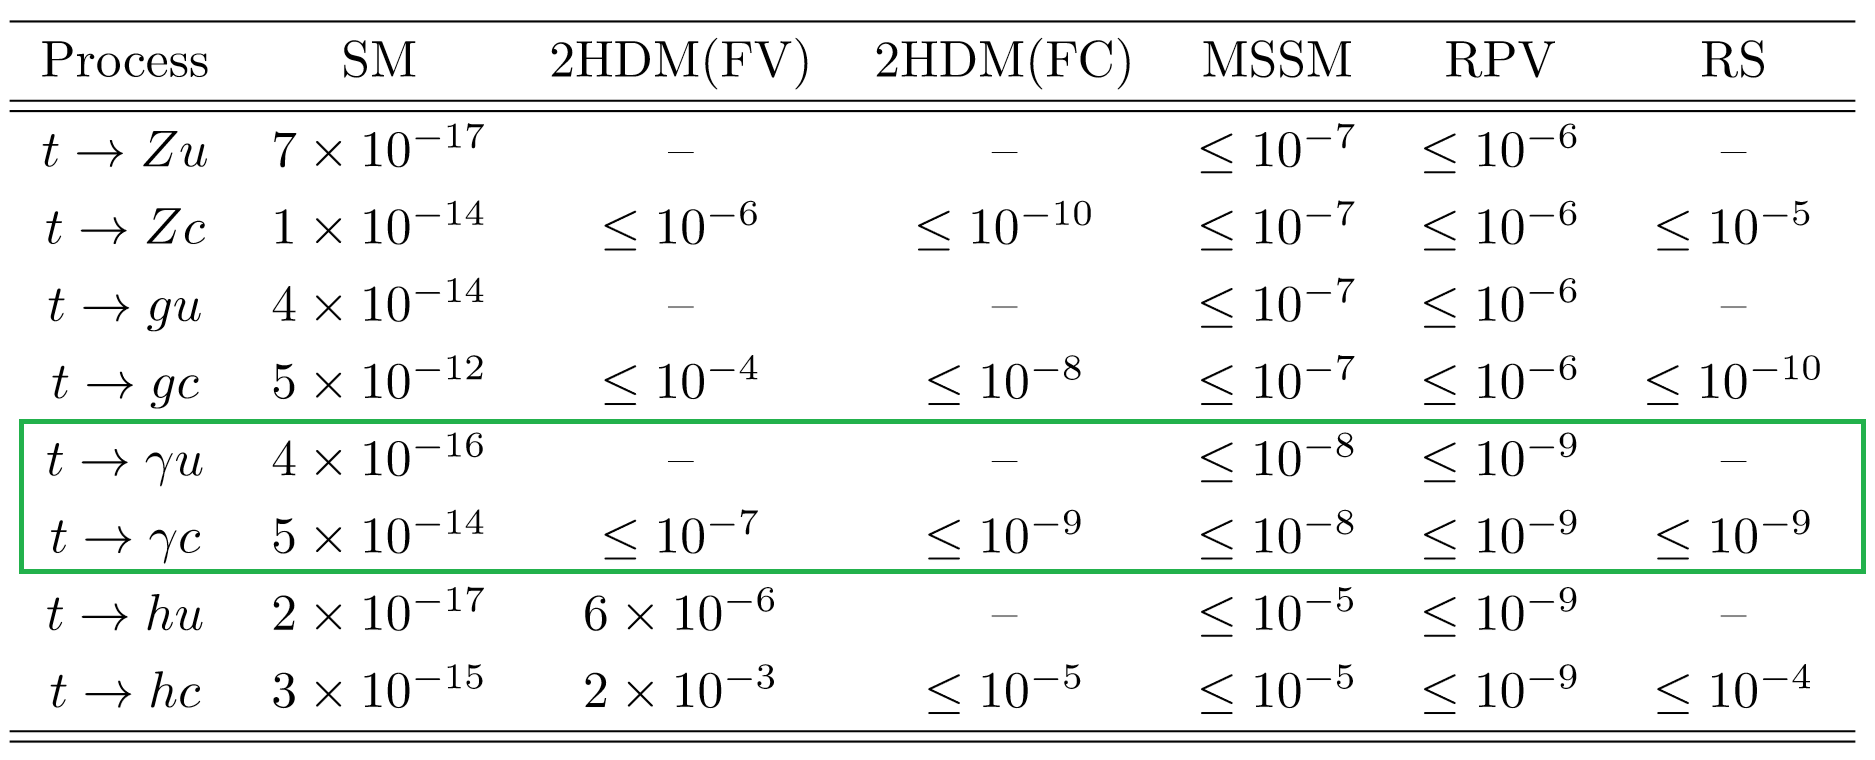
\includegraphics[width=1.\textwidth]{../../Thesis/ThesisImages/ModelLimits.png}
\captionof{table}{Branching ratio enhancements in various beyond the standard model theories \href{https://arxiv.org/pdf/1311.2028.pdf}{[Snowmass Top Report]}}

}

\frame{\frametitle{Top Flavor Changing Neutral Currents}
\begin{itemize}
\item Current Limits on FCNC Decays
\end{itemize}
\centering
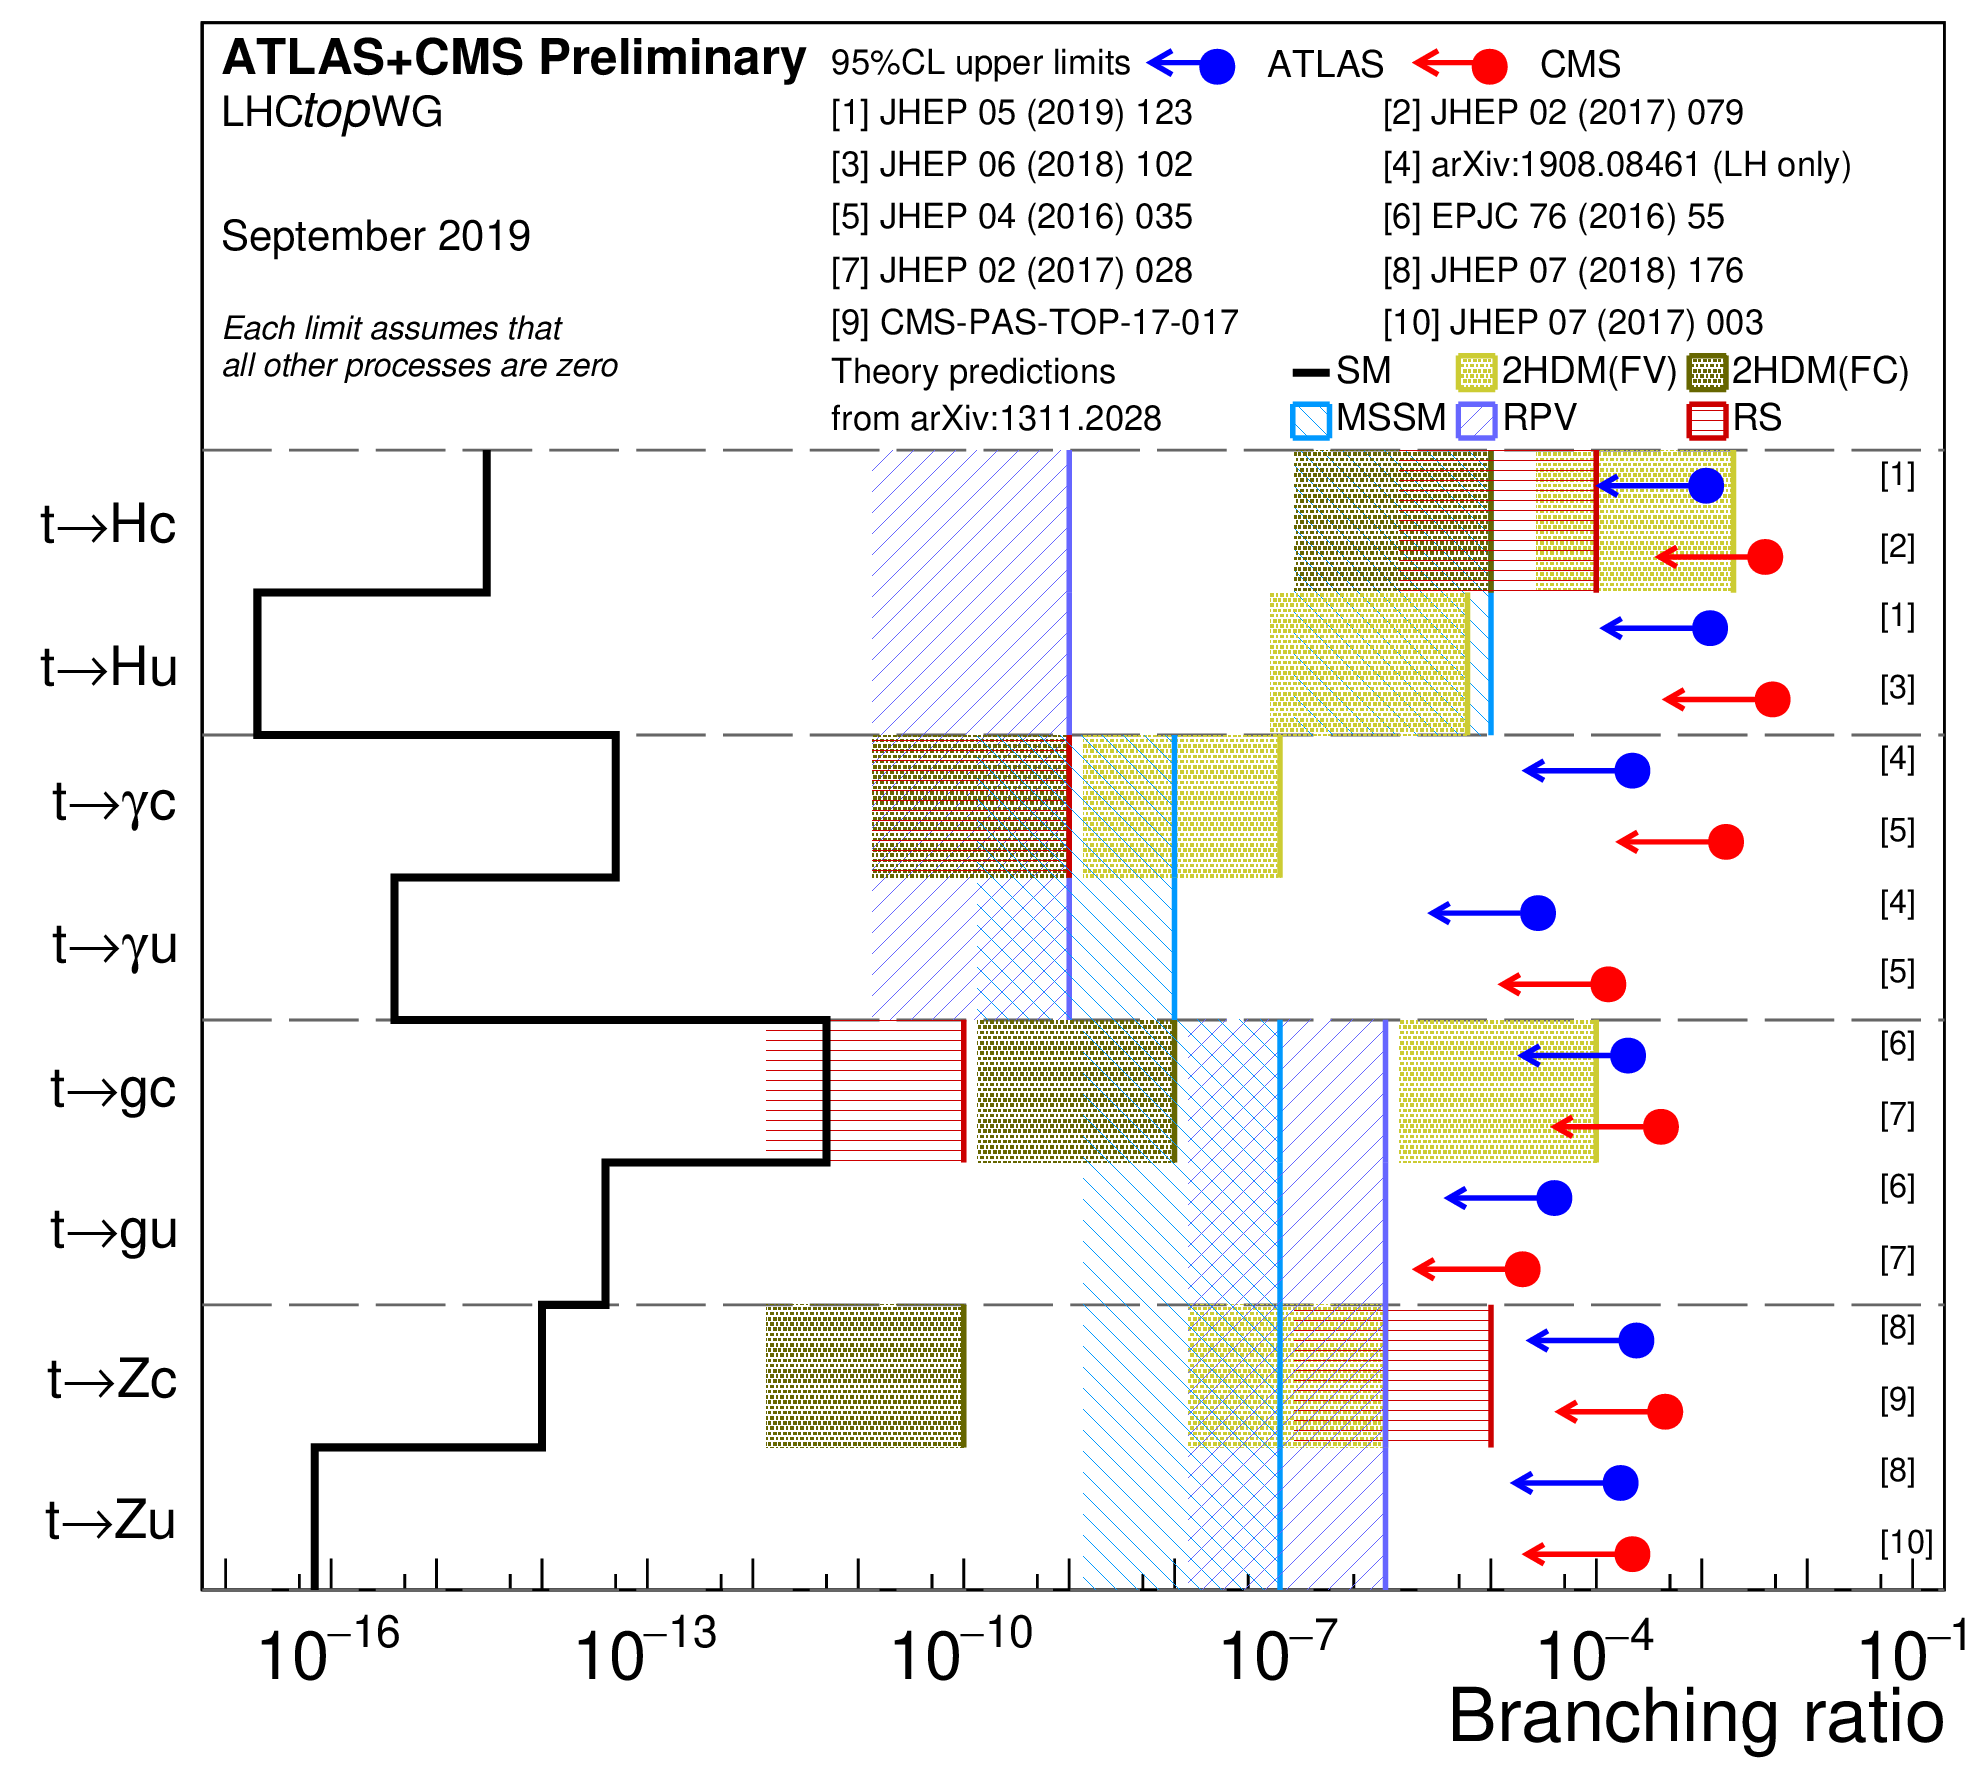
\includegraphics[width=0.55\textwidth]{../../Thesis/ThesisImages/Theory/AllFCNCLimits.png}
\begin{itemize}
\item Limits on $t\rightarrow \gamma q$ processes: \href{https://arxiv.org/abs/1908.08461}{arXiv:1908.08461}
	\begin{itemize}
	\item $t\rightarrow \gamma u < 6.1 x10^{-5}$
	\item $t\rightarrow \gamma c < 2.2 x 10^{-4}$
	\end{itemize}
\end{itemize}
}

\frame{\frametitle{Monte Carlo Production of FCNC Signal Samples}

\begin{itemize}
\item Due to the low cross sections we must create our own Monte Carlo Samples for our Signal
\item An effective field theory approach was taken in the creation of the model
\item This model takes advantage of dimension-6 operators
\end{itemize}
\[ \mathcal{L}_{SM} = \mathcal{L}_{SM}^{(4)} + \mathcal{L}^{eff} \text{ where } \mathcal{L}^{eff} = \frac{1}{\Lambda^2} \sum_{k} C_{k}^{(6)}Q_{k}^{(6)}
\]
\[ \mathcal{L}^{eff}_{tq\gamma} =  C \sigma^{\mu\nu}q_{\nu}(\lambda^{L}_{ct}P_L + \lambda^{R}_{ct}P_{R}) t A_{\mu} +H.c.
\]
}

%

\subsection{FCNC at the LHC}
\frame{\frametitle{FCNC: What are we looking for? $t\bar{t}\rightarrow W (\rightarrow l \nu) b+ q\gamma$}
\begin{itemize}
\item Final state topology
	\begin{itemize}
	\item One Neutrino, from W
	\item One Lepton, from W
	\item One B-jet, SM top
	\item One Photon, FCNC Top
	\item One Jet, FCNC Top
	\end{itemize}
\end{itemize}
\centering
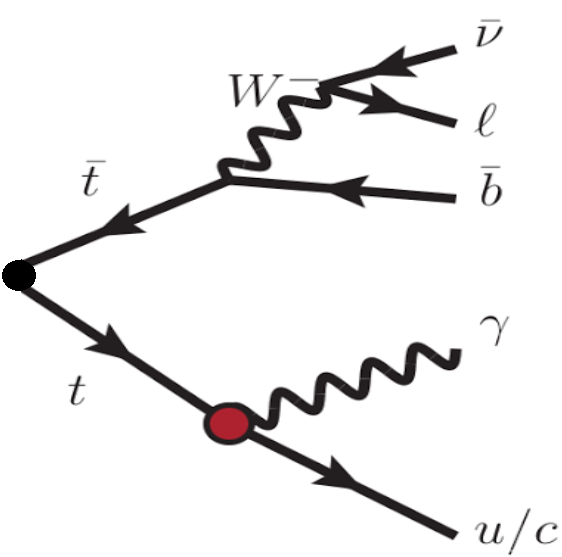
\includegraphics[width=0.4\textwidth]{../../Thesis/ThesisImages/fcncttbar.png}
}
%%%%%%%%%%%%%%%%%%%%%%%%%%%%%%%%%%%%%%%%%%%%%%%%%%%%%%

%%%%%%%%%%%%%%%%%%%%%%%%%%%%%%%%%%%%%%%%%%%%%%%%%%%%%%%%%%%%%%%%%%
\section{Flavor Changing Neutral Current Searches with Top Quarks}
\subsection{Object Preselection Cuts}


\frame{\frametitle{Object Preselection}
\begin{itemize}
\item We preselect events with objects that look like our expected topology
\item Require:
	\begin{itemize}
	\item Exactly one lepton (e or $\mu$) $\geq$ 25 GeV
	\item Exactly one Good photon $\geq$ 25GeV
	\item Missing Transverse Energy $\geq$ 30GeV
	\item $\geq 2$ Jets (at least one being b-tagged)
	\end{itemize}
\end{itemize}
}

\frame{\frametitle{Background Processes}
\begin{itemize}
\item Due to all of the processes at hadron colliders it is important to model similar event topologies well.
\item Major backgrounds include $t\bar{t}$, W+Jets, Z+Jets, + processes with an associated photon
\end{itemize}
\centering
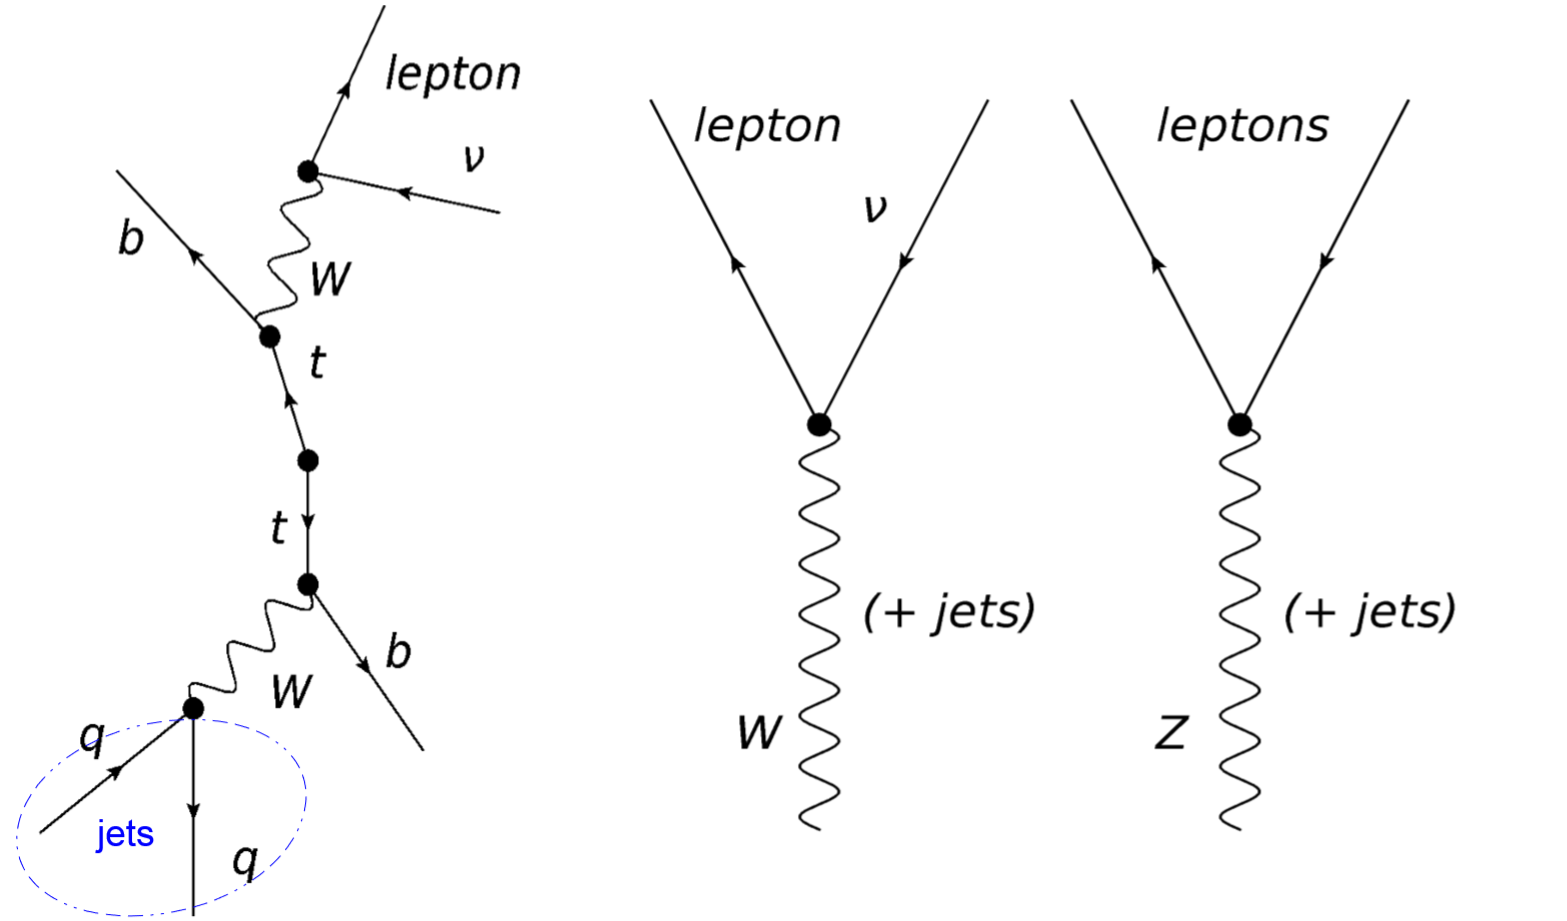
\includegraphics[width=0.7\textwidth]{../../Thesis/ThesisImages/backgrounds.png}
}

\frame{\frametitle{Preselection Objects}
Signal MC Scaled to 1\% $\sigma_{t\bar{t}}$, No Overlap Removal but no dedicated gamma samples
\begin{columns}
\begin{column}{0.02\textwidth}
\rotatebox{90}{Muon Channel \qquad  Electron Channel} 
%\rotatebox{90}{Muon Channel        } 
\end{column}
\begin{column}{0.33\textwidth}
\begin{itemize}
\item  Leading Jet $p_T$
\end{itemize}
\includegraphics[width=.95\textwidth]{Images/onlyNNCut/plotsSkip1percent/{el.presel.preselh_leadJet_pt}.png} \\
\includegraphics[width=.95\textwidth]{Images/onlyNNCut/plotsSkip1percent/{mu.presel.preselh_leadJet_pt}.png}
\end{column}
\begin{column}{0.33\textwidth}
\begin{itemize}
\item Lead Photon
\end{itemize}
\includegraphics[width=.95\textwidth]{Images/onlyNNCut/plotsSkip1percent/{el.presel.preselh_photon_pt}.png} \\
\includegraphics[width=.95\textwidth]{Images/onlyNNCut/plotsSkip1percent/{mu.presel.preselh_photon_pt}.png}
\end{column}
\begin{column}{0.33\textwidth}
\begin{itemize}
\item Lepton E
\end{itemize}
\includegraphics[width=.95\textwidth]{Images/onlyNNCut/plotsSkip1percent/{el.presel.preselh_lepton_pt}.png} \\
\includegraphics[width=.95\textwidth]{Images/onlyNNCut/plotsSkip1percent/{mu.presel.preselh_lepton_pt}.png}
\end{column}
\end{columns}
 No Overlap Removal but no dedicated gamma samples - Overall Scale Factors Needed
}

%%%%%%%%%%%%%%%%%%%%%%%%%%%%%%%%%%%%%%%%%%%%%%%%%%%%%%%%%%%%%%

\section{Neural Network}
\subsection{Neural Network Studies}

\frame{\frametitle{Neural Network Architecture}
\begin{itemize}
\item Using Keras on top of Tensorflow various input parameters are tested for model behavior
\item A Dense Neural Network with variable number of input variables and hidden layers are explored
\item Cut optimization has been performed with full Run 2 luminosity for potential reach of the search
\end{itemize}
\centering
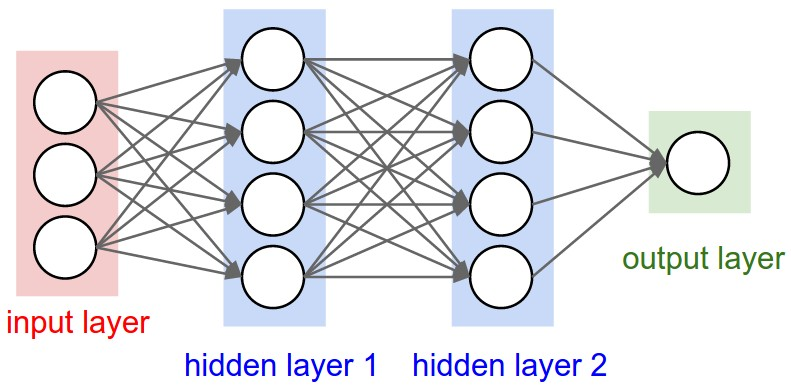
\includegraphics[width=0.7\textwidth]{Images/neural_net2.jpeg}
\captionof{figure}{\href{http://cs231n.github.io/neural-networks-1/}{[Ref: Neural Network]}}
}

\frame{\frametitle{Neural Network Model Inputs}
\begin{itemize}
\item Using keras on top of tensorflow various input parameters are tested for model behavior
\item Networks are set up with 1 input layer, 2 hidden layers with 10 nodes (+1 bias node) \href{https://www.quora.com/What-is-bias-in-artificial-neural-network}{[Ref: Bias]}, and 1 output node
\item Each hidden layer has 20\% dropout to prevent overtraining by removing codependency between nodes
\item Batch size of 100 used and each network is allowed 200 epochs (with patience=50), all models converge and end early with reasonable batch sizes
\item Optimizer: Adam
\item Loss Function: Binary Cross Entropy
\end{itemize}
}

\frame{\frametitle{Cut Optimization}
\begin{itemize}

\item  Reweighting the number of events the model saw by taking advantage of the loss function helps signal/background discrimination
\[\text{Loss} = -\frac{1}{N}\sum_{i=1}^{N}y_{i} \text{log}(p(y_{i}))+(1-y_{i})\text{log}(1-p(y_{i}))\]
\item y - binary indicator (0 or 1) if class label is the correct classification for observation 
\item p - predicted probability observation is the class label (0 or 1)
\end{itemize}
} 


\frame{\frametitle{Neural Network Example}
$\mu+$jets Channel Example

\begin{columns}
\begin{column}{0.33\textwidth}
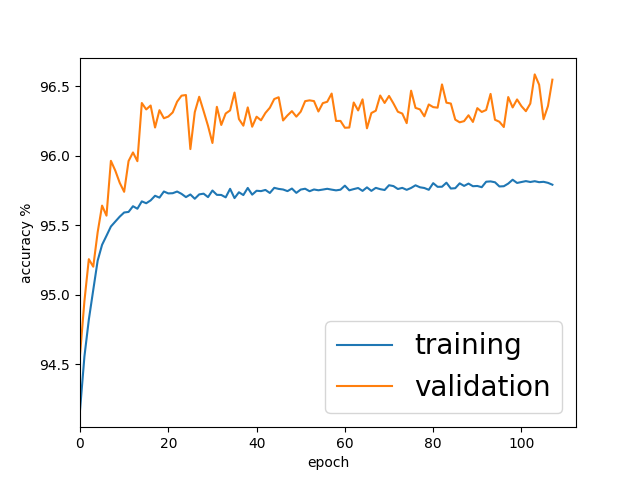
\includegraphics[width=.95\textwidth]{Images/SeptNN/accuarcy.png} \\
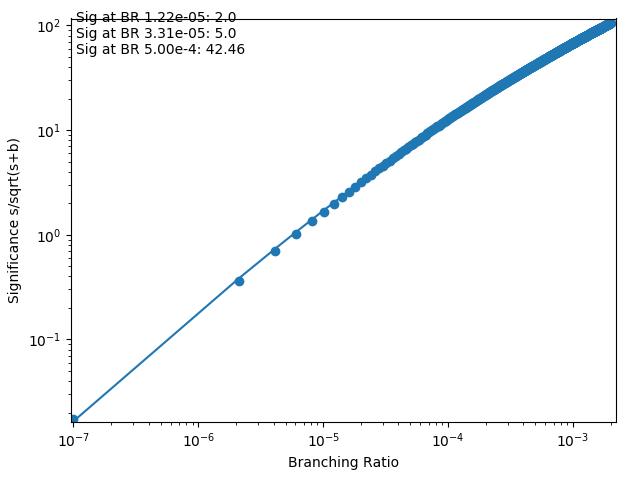
\includegraphics[width=.95\textwidth]{Images/SeptNN/SigVsBR.png}
\end{column}
\begin{column}{0.33\textwidth}

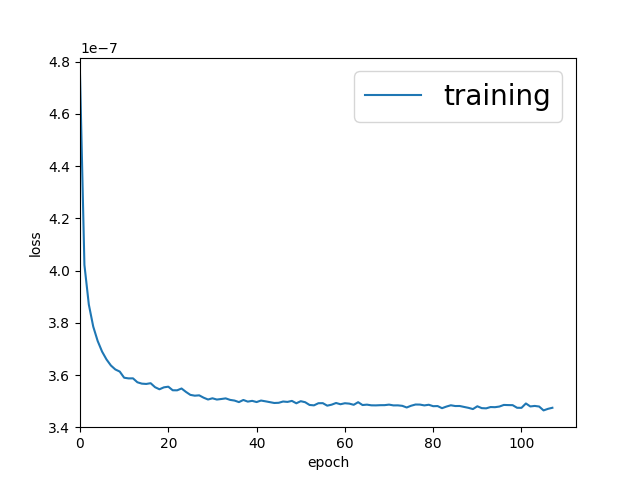
\includegraphics[width=.95\textwidth]{Images/SeptNN/loss.png} \\
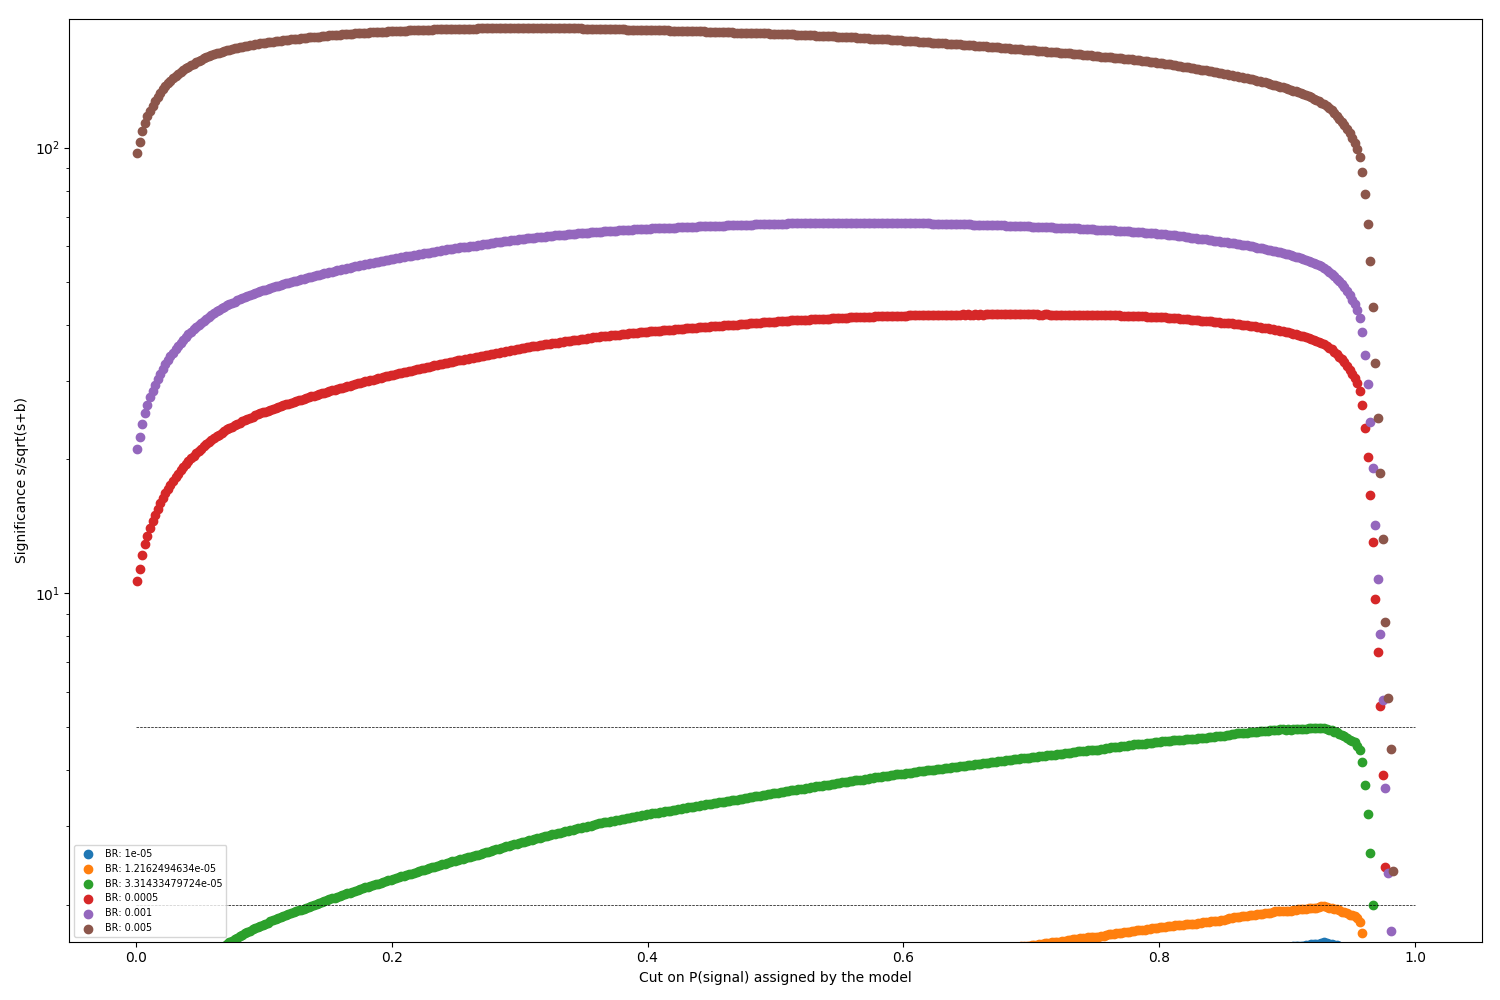
\includegraphics[width=.95\textwidth]{Images/SeptNN/significance2.png}
\end{column}
\begin{column}{0.33\textwidth}

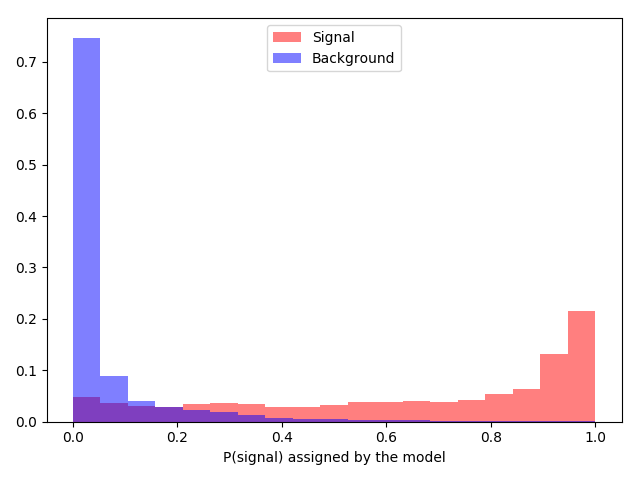
\includegraphics[width=.95\textwidth]{Images/SeptNN/sigbkg.png} \\
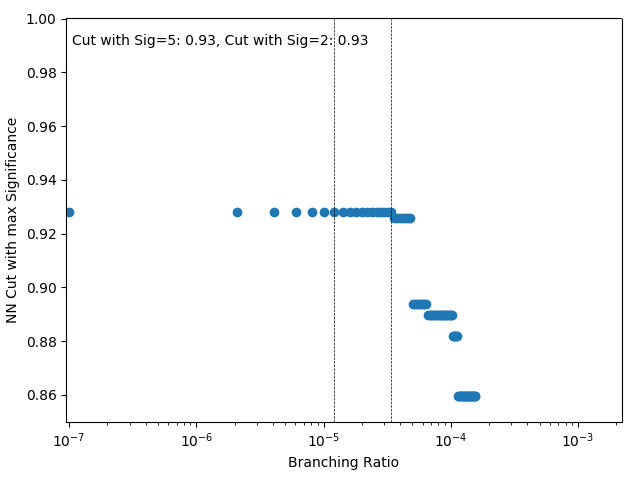
\includegraphics[width=.95\textwidth]{Images/SeptNN/CutVsBR.png}
\end{column}
\end{columns}
}

\frame{\frametitle{B-tagging}
\begin{columns}
\begin{column}{0.5\textwidth}
\begin{itemize}
\item B Hadrons travel a measureable distance before decay
\item Tracks originate from outside of interaction point (Seconday Vertex)
\item Backtracking tracks in displaced vertex gives an impact parameter
\item Decay chain MVA attempts to reconstruct decay of the jet
\item Outputs of these algorithms used in a BDT to determine if a Jet is from a b-quark
\end{itemize}
\end{column}
\begin{column}{0.5\textwidth}
\centering
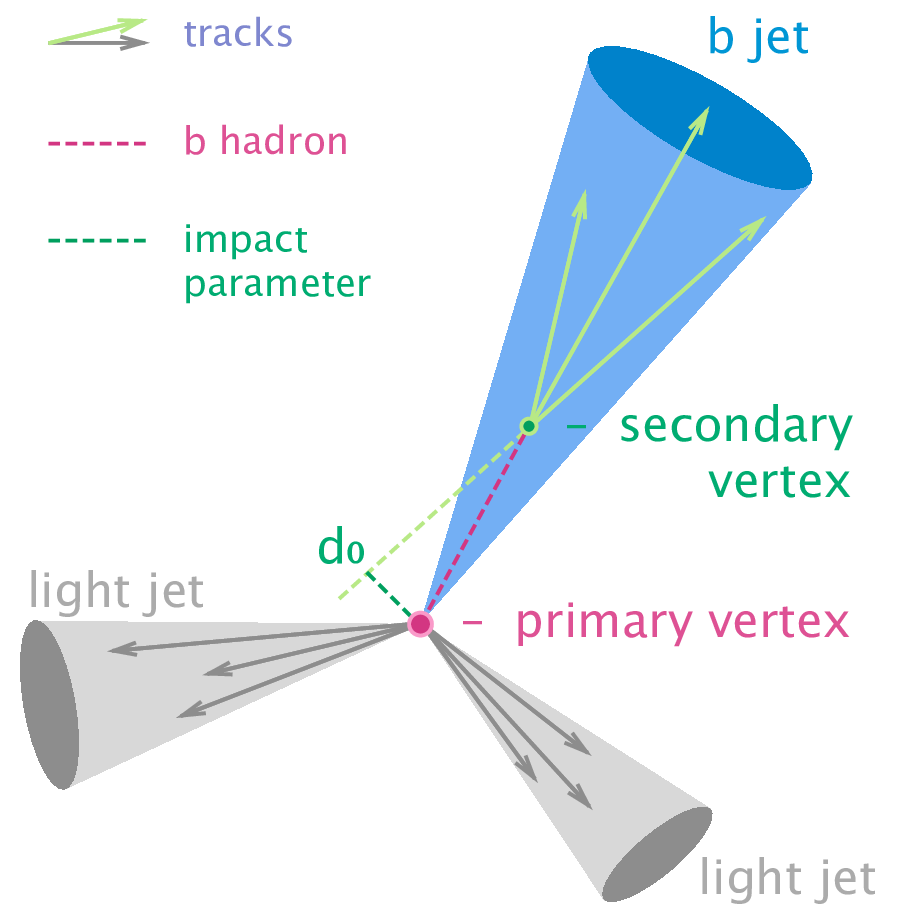
\includegraphics[height=.65\textheight]{../../Thesis/ThesisImages/Simulation/B-tagging_diagram.png}
\end{column}
\end{columns}
}


\frame{\frametitle{Neural Network B-Tagging Results}
\begin{columns}
\begin{column}{0.02\textwidth}
\rotatebox{90}{Muon Channel \qquad  Electron Channel} 
%\rotatebox{90}{Muon Channel        } 
\end{column}
\begin{column}{0.33\textwidth}
\begin{itemize}
\item  70\% Working Point
\end{itemize}
\includegraphics[width=.95\textwidth]{../../Thesis/ThesisImages/SimulationNN/{HiddenLayerStudiesBR0.002}/btag70/modelouts/significanceejetsboth2hidnpart02.png} \\
\tiny BR with Sig=2: $1.25\times10^{-5}$\\
\includegraphics[width=.95\textwidth]{../../Thesis/ThesisImages/SimulationNN/{HiddenLayerStudiesBR0.002}/btag70/modelouts/significancemujetsboth2hidnpart02.png}\\
BR with Sig=2: $1.31\times10^{-5}$
\end{column}
\begin{column}{0.33\textwidth}
\begin{itemize}
\item 77\% Working Point
\end{itemize}
\includegraphics[width=.95\textwidth]{../../Thesis/ThesisImages/SimulationNN/{HiddenLayerStudiesBR0.002}/btag77/modelouts/significanceejetsboth2hidnpart02.png} \\
\tiny BR with Sig=2: $1.23\times10^{-5}$\\
\includegraphics[width=.95\textwidth]{../../Thesis/ThesisImages/SimulationNN/{HiddenLayerStudiesBR0.002}/btag77/modelouts/significancemujetsboth2hidnpart02.png}\\
BR with Sig=2: $1.18\times10^{-5}$
\end{column}
\begin{column}{0.33\textwidth}
\begin{itemize}
\item 85\% Working Point
\end{itemize}
\includegraphics[width=.95\textwidth]{../../Thesis/ThesisImages/SimulationNN/{HiddenLayerStudiesBR0.002}/btag85/modelouts/significanceejetsboth2hidnpart02.png} \\
\tiny BR with Sig=2: $1.28\times10^{-5}$\\
\includegraphics[width=.95\textwidth]{../../Thesis/ThesisImages/SimulationNN/{HiddenLayerStudiesBR0.002}/btag85/modelouts/significancemujetsboth2hidnpart02.png}\\
BR with Sig=2: $1.19\times10^{-5}$
\end{column}
\end{columns}
}

\section{$e\rightarrow \gamma$ Fake Rate: Initial Studies}
\subsection{Initial Studies}

\frame{\frametitle{Fake Rate Studies}
\begin{centering}
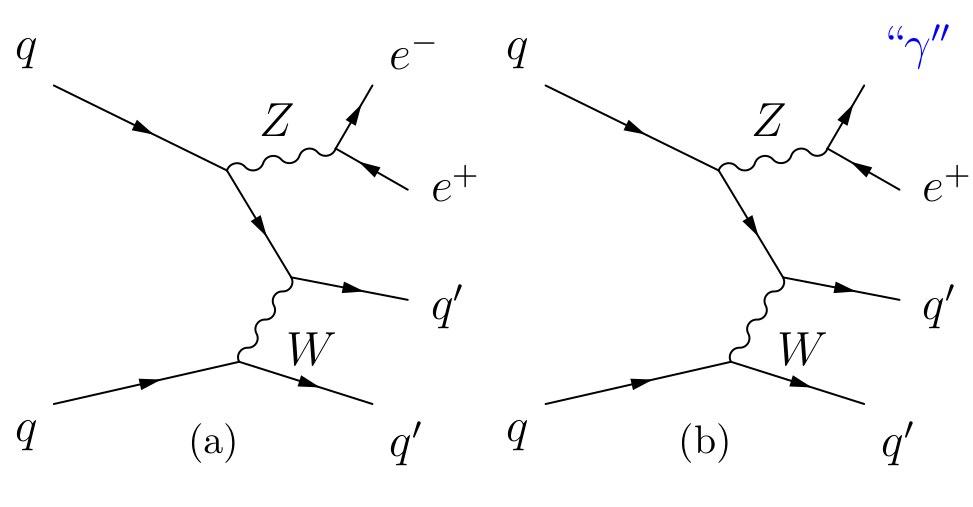
\includegraphics[width=.8\textwidth]{../../Thesis/ThesisImages/ZeeFakeDiagram.png}\\
\end{centering}
Want to be able to correct the number of fake photons predicted in MC to those present in Data
}

\subsection{Basic 1D Fake Rate Scale Factor}

\frame{Data and MC \frametitle{$m_{ee}, m_{e\gamma}$}
\begin{columns}
\begin{column}{0.02\textwidth}
\rotatebox{90}{$m_{e\gamma}$ \qquad \qquad \qquad $m_{ee}$\qquad} 
%\rotatebox{90}{Muon Channel        } 
\end{column}
\begin{column}{0.48\textwidth}
\begin{itemize}
\item Data
%\item  MCee integral small range: 424,051.  - Vgam: 429789 - All 430225
%\item DATAee integral small range: 468,832
%\item MCeg integral small range: 110822     - Vgam: 115066 - All 152420
%\item DATAeg integral small range: 118198
\end{itemize}
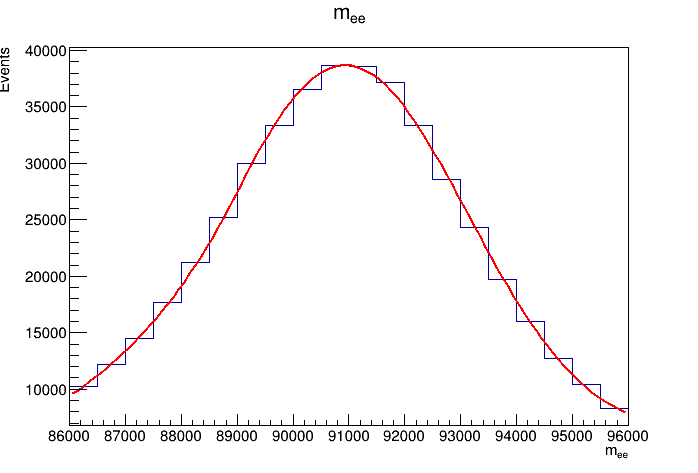
\includegraphics[width=.85\textwidth]{Images/Dataee.png} \\
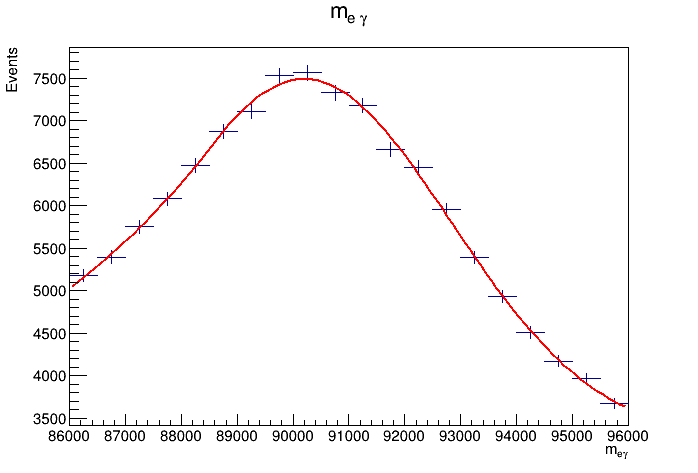
\includegraphics[width=.85\textwidth]{Images/Dataeg.png}
\end{column}
\begin{column}{0.48\textwidth}
\begin{itemize}
\item Monte Carlo
\end{itemize}
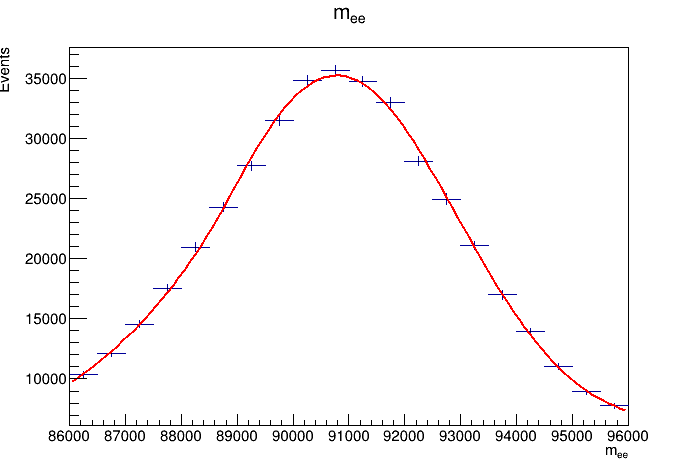
\includegraphics[width=.85\textwidth]{Images/MCVgamee.png} \\
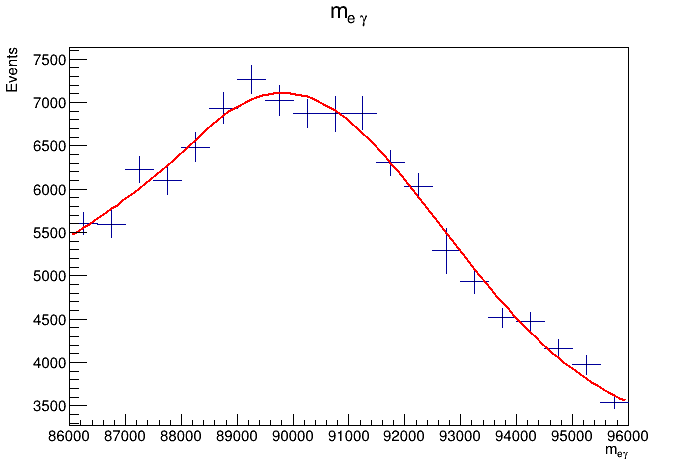
\includegraphics[width=.85\textwidth]{Images/MCVgameg.png}
\end{column}
\end{columns}
}


\frame{\frametitle{Scale Factor}
\[ \text{FR}^{\text{e-fake}}=\frac{N_{e,\gamma}}{N_{e,e}+N_{e,\gamma}}\]

\[  \text{SF}^{\text{e-fake}}_{\text{FR}} = \frac{\text{FR}^{\text{e-fake}}_{\text{data}}}{\text{FR}^{\text{e-fake}}_{\text{MC}}}\]
Basic Scale Factor can be calculated for the entire spectrum:
$\text{FR}^{\text{e-fake}}_{\text{data}} = 0.201$\\
$\text{FR}^{\text{e-fake}}_{\text{MC}} = 0.212$\\
$\text{SF}^{\text{e-fake}}_{\text{FR}} =0.953$
}

\frame{\frametitle{Scale Factors As Functions of Probe pt and eta}
\begin{columns}
\begin{column}{0.48\textwidth}
Probe $p_T$
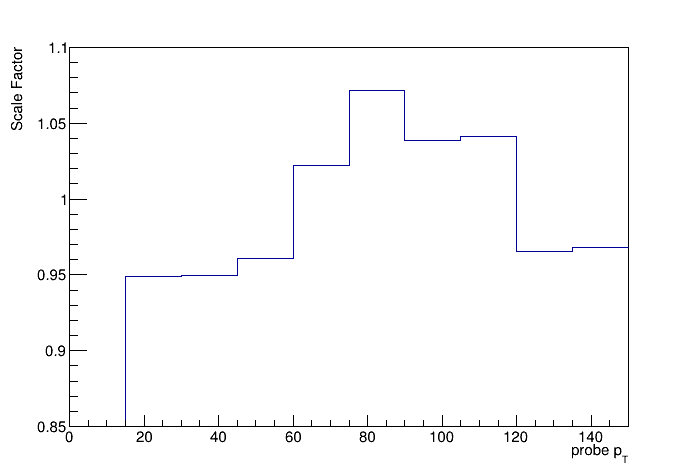
\includegraphics[width=\textwidth]{Images/pt1DSF.png}
\end{column}
\begin{column}{0.48\textwidth}
Probe $\eta$
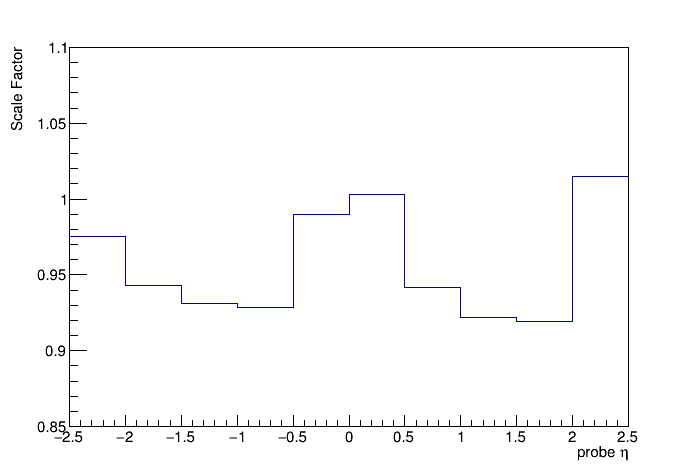
\includegraphics[width=\textwidth]{Images/eta1DSF.png}
\end{column}
\end{columns}
Good to check but in practice these are done using 2D Scale Factors
}

\subsection{2D Fake Rate Scale Factor}

\frame{\frametitle{Data and MC Distributions}
\begin{columns}
\begin{column}{0.02\textwidth}
\rotatebox{90}{ee region \qquad \qquad e$\gamma$ region\qquad} 
%\rotatebox{90}{Muon Channel        } 
\end{column}
\begin{column}{0.48\textwidth}
\begin{itemize}
\item Data
\end{itemize}
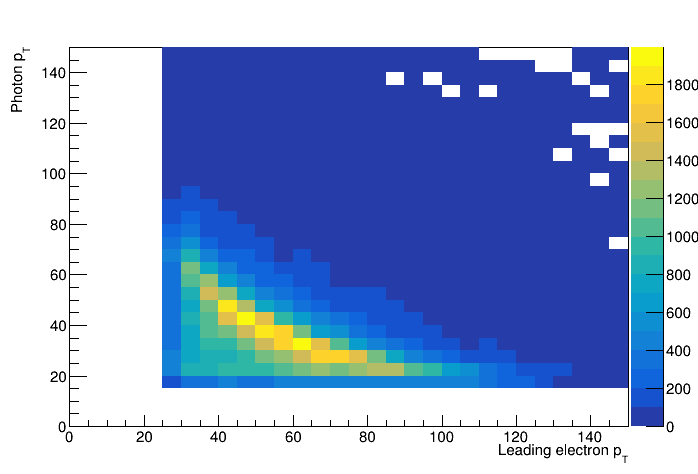
\includegraphics[width=.85\textwidth]{Images/dataPhotonElectronPT.png} \\
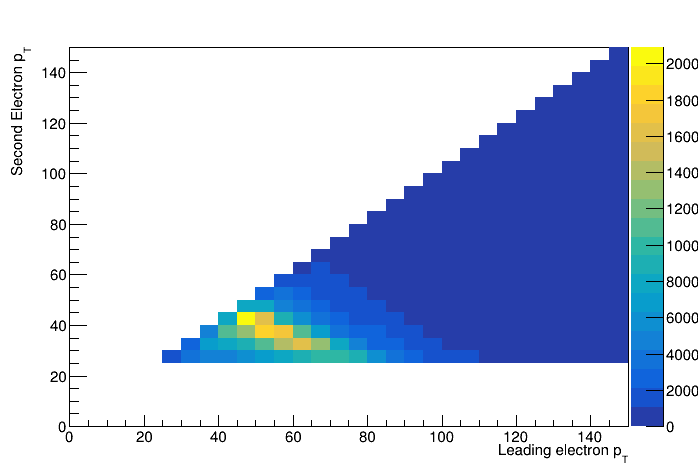
\includegraphics[width=.85\textwidth]{Images/dataElectronElectronPT.png}
\end{column}
\begin{column}{0.48\textwidth}
\begin{itemize}
\item Monte Carlo
\end{itemize}
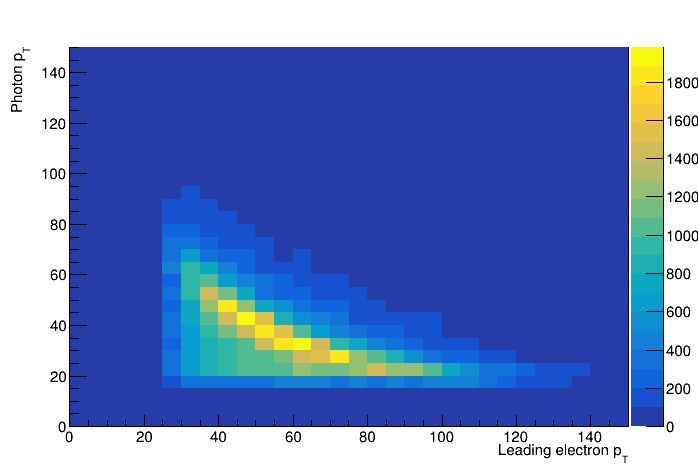
\includegraphics[width=.85\textwidth]{Images/mcPhotonElectronPT.png} \\
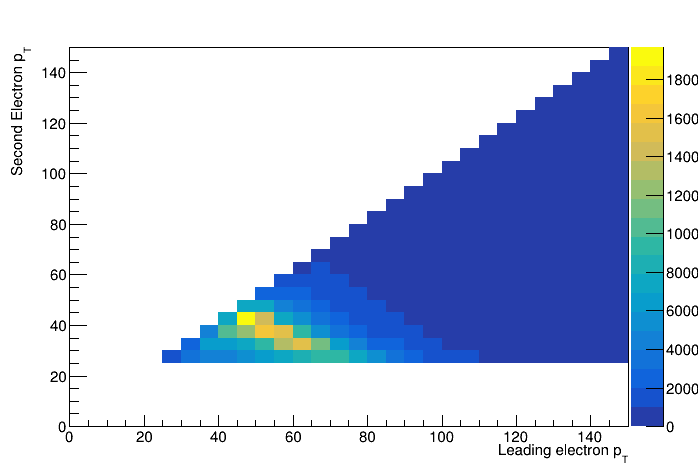
\includegraphics[width=.85\textwidth]{Images/mcElectronElectronPT.png}
\end{column}
\end{columns}
}

\frame{\frametitle{2D Fake Rate}
\centering
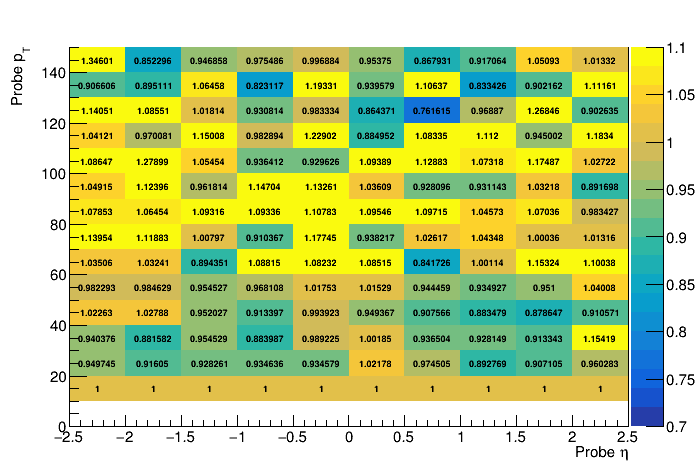
\includegraphics[width=.95\textwidth]{Images/2DSF.png}\\
Fake rate will be recalculated using the newest ntuples soon
}
\section{First Analysis Plots}

\frame{\frametitle{Analysis Plots}
\begin{table}[]
\tiny
\begin{tabular}{lllllll} \hline
 		&	VR1:$W+\gamma$	 & VR2:$t\bar{t}+\gamma$	& VR3:$t\bar{t}$/W+Jets   & CR1: W+Jets Rich  & CR2: $t\bar{t}$ Rich & SR  \\ \hline \\
$n_{\gamma}$&	=1	 & =1	   & =0 &= 0 & =0 & =1  \\ \hline \\
$n_{\text{jet}}$&	$\geq$2	 & $\geq$4  & =4 & =3  & $\geq$5  & $\geq$2  \\ \hline \\
$n_{b_{\text{jet}}}$&=0	 & =1 	   & =1 &  =1 &  =1 & =1  \\ \hline \\
$n_{\text{lepton}}$& =1& =1 & =1 & =1& =1 & =1 \\ \hline \\
Neural Network Cut &-	 &  $<$NNCut	& - & - & -  & $>$NNCut  \\ \hline \\
\end{tabular}
\end{table}
Additional cuts are employed as well to slim out certain backgrounds.
The following plots are for MC16a and Data 2015/2016, signal is scaled to 1\% $\sigma_{t\bar{t}}$ except for SR where it is scaled to $0.01\%\sigma_{t\bar{t}}$ 
}



\frame{\frametitle{VR1: $W+\gamma$ VR Plots - $m_{T}^W$, lepton $p_{T}$, $S_T$}
\begin{columns}
\begin{column}{0.02\textwidth}
\rotatebox{90}{Muon Channel \qquad  Electron Channel} 
%\rotatebox{90}{Muon Channel        } 
\end{column}
\begin{column}{0.33\textwidth}
\includegraphics[width=.9\textwidth]{Images/Plots/{FCNCplots1percent}/ejets/Plots/VR1_MWT.png} \\
\includegraphics[width=.9\textwidth]{Images/Plots/{FCNCplots1percent}/mujets/Plots/VR1_MWT.png}\\
\end{column}
\begin{column}{0.33\textwidth}
\includegraphics[width=.9\textwidth]{Images/Plots/{FCNCplots1percent}/ejets/Plots/VR1_lep_pt.png} \\
\includegraphics[width=.9\textwidth]{Images/Plots/{FCNCplots1percent}/mujets/Plots/VR1_lep_pt.png}\\
\end{column}
\begin{column}{0.33\textwidth}
\includegraphics[width=.9\textwidth]{Images/Plots/{FCNCplots1percent}/ejets/Plots/VR1_ST.png} \\
\includegraphics[width=.9\textwidth]{Images/Plots/{FCNCplots1percent}/mujets/Plots/VR1_ST.png}\\
\end{column}
\end{columns}
}

\frame{\frametitle{VR2: $t\bar{t}+\gamma$ VR Plots - $m_{T}^W$, lepton $p_{T}$, $m_{Wb}$}
\begin{columns}
\begin{column}{0.02\textwidth}
\rotatebox{90}{Muon Channel \qquad  Electron Channel} 
%\rotatebox{90}{Muon Channel        } 
\end{column}
\begin{column}{0.33\textwidth}
\includegraphics[width=.9\textwidth]{Images/Plots/{FCNCplots1percent}/ejets/Plots/VR2_MWT.png} \\
\includegraphics[width=.9\textwidth]{Images/Plots/{FCNCplots1percent}/mujets/Plots/VR2_MWT.png}\\
\end{column}
\begin{column}{0.33\textwidth}
\includegraphics[width=.9\textwidth]{Images/Plots/{FCNCplots1percent}/ejets/Plots/VR2_lep_pt.png} \\
\includegraphics[width=.9\textwidth]{Images/Plots/{FCNCplots1percent}/mujets/Plots/VR2_lep_pt.png}\\
\end{column}
\begin{column}{0.33\textwidth}
\includegraphics[width=.9\textwidth]{Images/Plots/{FCNCplots1percent}/ejets/Plots/VR2_SMtop.png} \\
\includegraphics[width=.9\textwidth]{Images/Plots/{FCNCplots1percent}/mujets/Plots/VR2_SMtop.png}\\
\end{column}
\end{columns}
}

\frame{\frametitle{W+Jets Rich CR Plots - $m_{T}^W$, lepton $p_{T}$, $m_{Wb}$}
\begin{columns}
\begin{column}{0.02\textwidth}
\rotatebox{90}{Muon Channel \qquad  Electron Channel} 
%\rotatebox{90}{Muon Channel        } 
\end{column}
\begin{column}{0.33\textwidth}
\includegraphics[width=.9\textwidth]{Images/Plots/{FCNCplots1percent}/ejets/Plots/CR1_MWT.png} \\
\includegraphics[width=.9\textwidth]{Images/Plots/{FCNCplots1percent}/mujets/Plots/CR1_MWT.png}\\
\end{column}
\begin{column}{0.33\textwidth}
\includegraphics[width=.9\textwidth]{Images/Plots/{FCNCplots1percent}/ejets/Plots/CR1_lep_pt.png} \\
\includegraphics[width=.9\textwidth]{Images/Plots/{FCNCplots1percent}/mujets/Plots/CR1_lep_pt.png}\\
\end{column}
\begin{column}{0.33\textwidth}
\includegraphics[width=.9\textwidth]{Images/Plots/{FCNCplots1percent}/ejets/Plots/CR1_SMtop.png} \\
\includegraphics[width=.9\textwidth]{Images/Plots/{FCNCplots1percent}/mujets/Plots/CR1_SMtop.png}\\
\end{column}
\end{columns}
}

\frame{\frametitle{$t\bar{t}$ Rich CR Plots - $m_{T}^W$, lepton $p_{T}$, $m_{Wb}$}
\begin{columns}
\begin{column}{0.02\textwidth}
\rotatebox{90}{Muon Channel \qquad  Electron Channel} 
%\rotatebox{90}{Muon Channel        } 
\end{column}
\begin{column}{0.33\textwidth}
\includegraphics[width=.9\textwidth]{Images/Plots/{FCNCplots1percent}/ejets/Plots/CR2_MWT.png} \\
\includegraphics[width=.9\textwidth]{Images/Plots/{FCNCplots1percent}/mujets/Plots/CR2_MWT.png}\\
\end{column}
\begin{column}{0.33\textwidth}
\includegraphics[width=.9\textwidth]{Images/Plots/{FCNCplots1percent}/ejets/Plots/CR2_lep_pt.png} \\
\includegraphics[width=.9\textwidth]{Images/Plots/{FCNCplots1percent}/mujets/Plots/CR2_lep_pt.png}\\
\end{column}
\begin{column}{0.33\textwidth}
\includegraphics[width=.9\textwidth]{Images/Plots/{FCNCplots1percent}/ejets/Plots/CR2_SMtop.png} \\
\includegraphics[width=.9\textwidth]{Images/Plots/{FCNCplots1percent}/mujets/Plots/CR2_SMtop.png}\\
\end{column}
\end{columns}
}



\frame{\frametitle{$t\bar{t}$/W+Jets VR Plots - $m_{T}^W$, lepton $p_{T}$, $m_{Wb}$}
\begin{columns}
\begin{column}{0.02\textwidth}
\rotatebox{90}{Muon Channel \qquad  Electron Channel} 
%\rotatebox{90}{Muon Channel        } 
\end{column}
\begin{column}{0.33\textwidth}
\includegraphics[width=.9\textwidth]{Images/Plots/{FCNCplots1percent}/ejets/Plots/VR3_MWT.png} \\
\includegraphics[width=.9\textwidth]{Images/Plots/{FCNCplots1percent}/mujets/Plots/VR3_MWT.png}\\
\end{column}
\begin{column}{0.33\textwidth}
\includegraphics[width=.9\textwidth]{Images/Plots/{FCNCplots1percent}/ejets/Plots/VR3_lep_pt.png} \\
\includegraphics[width=.9\textwidth]{Images/Plots/{FCNCplots1percent}/mujets/Plots/VR3_lep_pt.png}\\
\end{column}
\begin{column}{0.33\textwidth}
\includegraphics[width=.9\textwidth]{Images/Plots/{FCNCplots1percent}/ejets/Plots/VR3_SMtop.png} \\
\includegraphics[width=.9\textwidth]{Images/Plots/{FCNCplots1percent}/mujets/Plots/VR3_SMtop.png}\\
\end{column}
\end{columns}
}

\frame{\frametitle{SR Plots - $m_{T}^W$, lepton $p_{T}$, $m_{Wb}$}
\begin{columns}
\begin{column}{0.02\textwidth}
\rotatebox{90}{Muon Channel \qquad  Electron Channel} 
%\rotatebox{90}{Muon Channel        } 
\end{column}
\begin{column}{0.33\textwidth}
\includegraphics[width=.9\textwidth]{Images/Plots/{FCNCplots0.01percent}/ejets/Plots/SR_MWT.png} \\
\includegraphics[width=.9\textwidth]{Images/Plots/{FCNCplots0.01percent}/mujets/Plots/SR_MWT.png}\\
\end{column}
\begin{column}{0.33\textwidth}
\includegraphics[width=.9\textwidth]{Images/Plots/{FCNCplots0.01percent}/ejets/Plots/SR_lep_pt.png} \\
\includegraphics[width=.9\textwidth]{Images/Plots/{FCNCplots0.01percent}/mujets/Plots/SR_lep_pt.png}\\
\end{column}
\begin{column}{0.33\textwidth}
\includegraphics[width=.9\textwidth]{Images/Plots/{FCNCplots0.01percent}/ejets/Plots/SR_SMtop.png} \\
\includegraphics[width=.9\textwidth]{Images/Plots/{FCNCplots0.01percent}/mujets/Plots/SR_SMtop.png}\\
\end{column}
\end{columns}
}

\frame{\frametitle{SR Plots - $S_T$, $\gamma$ $p_{T}$, $m_{q\gamma}$}
\begin{columns}
\begin{column}{0.02\textwidth}
\rotatebox{90}{Muon Channel \qquad  Electron Channel} 
%\rotatebox{90}{Muon Channel        } 
\end{column}
\begin{column}{0.33\textwidth}
\includegraphics[width=.9\textwidth]{Images/Plots/{FCNCplots0.01percent}/ejets/Plots/SR_ST.png} \\
\includegraphics[width=.9\textwidth]{Images/Plots/{FCNCplots0.01percent}/mujets/Plots/SR_ST.png}\\
\end{column}
\begin{column}{0.33\textwidth}
\includegraphics[width=.9\textwidth]{Images/Plots/{FCNCplots0.01percent}/ejets/Plots/SR_ph_pt.png} \\
\includegraphics[width=.9\textwidth]{Images/Plots/{FCNCplots0.01percent}/mujets/Plots/SR_ph_pt.png}\\
\end{column}
\begin{column}{0.33\textwidth}
\includegraphics[width=.9\textwidth]{Images/Plots/{FCNCplots0.01percent}/ejets/Plots/SR_mqph.png} \\
\includegraphics[width=.9\textwidth]{Images/Plots/{FCNCplots0.01percent}/mujets/Plots/SR_mqph.png}\\
\end{column}
\end{columns}
}

\frame{\frametitle{To-Do}
\begin{itemize}
\item Need to apply Z-Mass Cut to SR
\item
\item
\end{itemize}
}

\frame{\frametitle{Timeline}
\begin{itemize}
\item
\item
\item
\end{itemize}
}

\subsection{Conclusion}
\frame{\frametitle{Conclusion}
\begin{itemize}
\item An excess signal would be indicative of some physics beyond the Standard Mode that couples strongly to the top sector
\item The search for FCNCs with enhanced rates are important pieces of testing many new theories
\item Barring any excess: with $\approx 138 \text{fb}^{-1}$ data at $\sqrt{s}=$ 13TeV setting an upper limit of  $\text{BR}(t\rightarrow q \gamma) <  3x10^{-5}$ is a reasonable goal, extrapolating from past results. 
\end{itemize}
}
%
%
%\frame{\frametitle{Reconstructed Tops}
%\begin{columns}
%\begin{column}{0.02\textwidth}
%\rotatebox{90}{Muon Channel \qquad  Electron Channel} 
%\end{column}
%\begin{column}{0.5\textwidth}
%\begin{itemize}
%\item SM Top
%\end{itemize}
%\centering
%\includegraphics[width=.9\textwidth]{../../ThesisImages/plotsloose/el_h_sm_top_m.png}\\
%\includegraphics[width=.9\textwidth]{../../ThesisImages/plotsloose/mu_h_sm_top_m.png}
%\end{column} 
%\begin{column}{0.5\textwidth}
%\begin{itemize}
%\item FCNC Top
%\end{itemize}
%\centering
%\includegraphics[width=.9\textwidth]{../../ThesisImages/plotsloose/el_h_qgam_m.png}\\
%\includegraphics[width=.9\textwidth]{../../ThesisImages/plotsloose/mu_h_qgam_m.png}
%\end{column}
%\end{columns}
%}

%
%
%%%%%%%%%%%%%%%%%%%%%%%%%%%%%%%%%%%%%%%%%%%%%%%%%%%%%%%%%%%%%%%%%%%
%\section{}
%\subsection{Outlook}
%\frame{\frametitle{Outlook}
%\begin{itemize}
%\item Many improvements can be made to the analysis
%\begin{itemize}
%\item Investigation of $\chi^2$ as a discriminating variable
%\item Inclusion of isolation and spatial proximity cuts
%\end{itemize}
%\item Monte Carlo distributions can be used to set an expected limit on the Branching Ratio
%\end{itemize}
%\centering
%\includegraphics[width=.5\textwidth]{../../ThesisImages/plotsstrict/el_h_min_chi2.png}
%\captionof{figure}{e-channel $\chi^2$ after Z, Bjet cuts}
%}
%
%

%}
%

%%%%%%%%%%%%%%%%%%%%%%%%%%%%%%%%%%%%%%%%%%%%%%%%%%%%%%%%%%%%%%%%

\appendix
\section{Backup}
\frame{\frametitle{Backup}
}

\frame{\frametitle{Neural Network Model Inputs}
\centering
\scalebox{0.8}{ $\text{Separation} = \sum_{i}^{bins} \frac {n_{s i}-n_{b i}}{n_{s i}+n_{b i}}$}
\begin{columns}
\begin{column}{0.48\textwidth}
\centering
mu+jets channel\\
\scalebox{0.6}{\begin{tabular}{cc}
Variable & Separation \\
\hline
photon0iso & 41.18 \\
mqgam & 28.27 \\
photon0pt & 24.07 \\
mtSM & 11.60 \\
mlgam & 7.56 \\
deltaRjgam & 5.64 \\
deltaRbl & 4.42 \\
MWT & 3.34 \\
ST & 3.30 \\
nuchi2 & 3.12 \\
jet0pt & 2.81 \\
njets & 2.07 \\
smchi2 & 1.89 \\
wchi2 & 1.87 \\
jet0e & 1.52 \\
deltaRlgam & 1.17 \\
leptone & 0.87 \\
deltaRjb & 0.86 \\
met & 0.68 \\
bjet0pt & 0.52 \\
leptoniso & 0.27 \\
\end{tabular}
}
\end{column}
\begin{column}{0.48\textwidth}
\centering
e+jets channel \\
\scalebox{0.6}{\begin{tabular}{c c}
Variable & Separation\\
\hline
photon0pt & 23.14 \\
mqgam & 22.73 \\
photon0iso & 18.70 \\
mtSM & 11.02 \\
mlgam & 9.53 \\
deltaRbl & 5.00 \\
deltaRjgam & 4.60 \\
ST & 3.83 \\
MWT & 3.16 \\
jet0pt & 2.47 \\
njets & 1.70 \\
nuchi2 & 1.59 \\
deltaRlgam & 1.40 \\
wchi2 & 1.33 \\
smchi2 & 1.09 \\
deltaRjb & 0.88 \\
leptone & 0.85 \\
leptoniso & 0.56 \\
bjet0pt & 0.50 \\
met & 0.47 \\
\end{tabular}
}
\end{column}
\end{columns}
}

\frame{\frametitle{Input Variables}
['photon0iso','photon0pt','mqgam','mlgam','mtSM','deltaRjgam','deltaRbl',\\
'MWT','ST','njets','wchi2','jet0pt','deltaRlgam','leptone','met','bjet0pt']
}

\frame{\frametitle{FCNC Diagrams}
\centering
\includegraphics[width=.4\textwidth]{../../Thesis/ThesisImages/Theory/FCNCLoop.png}
\includegraphics[width=.4\textwidth]{../../Thesis/ThesisImages/penguinFCNC.png}
}
\frame{\frametitle{A Couple of BSM Diagrams}
\centering
\includegraphics[width=1.\textwidth]{../../Thesis/ThesisImages/BSMDiagrams.png}
}

\frame{\frametitle{Jets/AntiKT}

\[ d_{ij} = min(\frac{1}{p_{ti}^2},\frac{1}{p_{tj}^2}) \frac{\Delta_{ij}^2}{R^2}
\]
\[ d_{iB} = \frac{1}{p_{ti}^2}
\]
\[ \Delta_{ij}^2 = (\eta_i -\eta_j )^2 + (\phi_i - \phi_j )^2
\]
\begin{itemize}
\item Find minimum of entire set of $\{ d_{ij},d_{iB} \}$
\item If $d_{ij}$ is the minimum particles i,j are combined into one particle and removed from the list of particles
\item If $d_{iB}$ is the minimum i is labelled as a final jet and removed from the list of particles
\item Repeat until all particles are part of a jet with distance between jet axes $\Delta_{ij}$ is greater than R
\end{itemize}
}

\frame{\frametitle{B-tagging}
\centering
\includegraphics[height=.8\textheight]{../../Thesis/ThesisImages/Simulation/B-tagging_diagram.png}
}

\frame{\frametitle{}
\[ \mathcal{L}^{eff}_{tq\gamma} = - e \bar{c} \frac{i \sigma^{\mu\nu}q_{\nu}}{m_t}(\lambda^{L}_{ct}P_L + \lambda^{R}_{ct}P_{R}) t A_{\mu} +H.c.
\]
}



\end{document}
%
%%36.070
